% ©SHRVAN NANDER PANDALA S5 CS2
\documentclass{article}
\usepackage{amsmath}
\usepackage{geometry}
\usepackage{listings}
\usepackage{fancyvrb}
\usepackage{multicol}
\usepackage{graphicx}
\usepackage{caption}
\usepackage{tikz}
\usepackage{eso-pic}
\usepackage{array}
\usepackage{afterpage}
\usepackage{float}

\geometry{a4paper, left=0.75in, right=0.75in, top=0.65in, bottom=0.25in}
\pagestyle{empty}
\pagenumbering{gobble}

% Define the border and header drawing command
\newcommand\PageBorder{%
  \begin{tikzpicture}[remember picture,overlay]
    % Date Label (top left)
    \node[anchor=north west, font=\large] 
      at ([xshift=0.75in,yshift=-0.25in]current page.north west) {Date:\hspace{3cm}};
    % Page No Label (top right)
    \node[anchor=north east, font=\large] 
      at ([xshift=-1.25in,yshift=-0.25in]current page.north east) {Page No:\hspace{2.5cm}};
  \end{tikzpicture}% % <-- pushes text down
}
\AddToShipoutPicture{\PageBorder}

%dont edit anything above............


\begin{document}
\section*{\centering{Cycle 1}}
\begin{figure}[H]
    \centering
    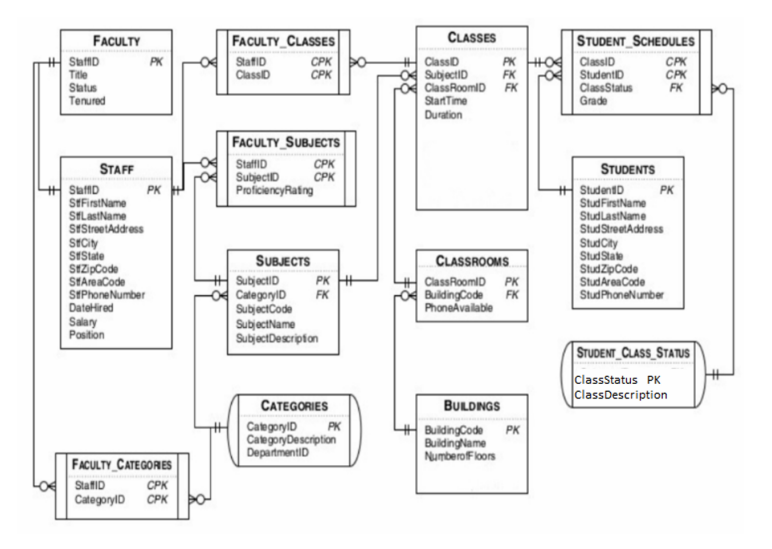
\includegraphics[width=0.95\textwidth]{cycle1/1.png}
    \label{fig:schema}
\end{figure}

\subsection*{1.  Design the ER diagram from the given schema.}
\begin{figure}[H]
    \centering
    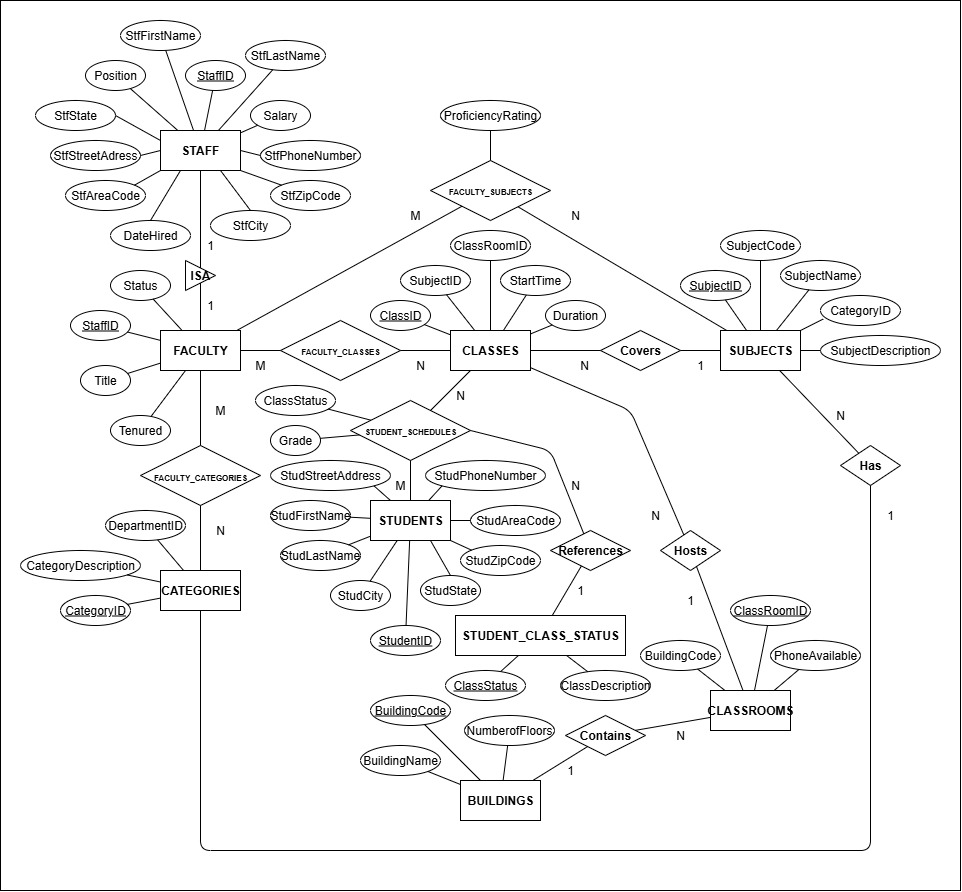
\includegraphics[width=0.8\textwidth]{cycle1/ER.jpeg}
    \label{fig:schema}
\end{figure}
\subsection*{2. Create the database with proper tables, columns, column types and \\
constraints.}

\subsubsection*{Staff Table}
Query:
\begin{Verbatim}[frame=single,framerule=1pt,fontfamily=courier,fontsize=\small]
CREATE TABLE STAFF (
StaffID INT PRIMARY KEY,
StfFirstName VARCHAR(30) NOT NULL,
StfLastName VARCHAR(30) NOT NULL,
StfStreetAddress VARCHAR(30) NOT NULL,
StfCity VARCHAR(30) NOT NULL,
StfState VARCHAR(30) NOT NULL,
StfZipCode INT NOT NULL,
StfAreaCode INT NOT NULL,
StfPhoneNumber INT NOT NULL,
DateHired DATE NOT NULL,
Salary INT NOT NULL,
Position VARCHAR(30) NOT NULL
);
\end{Verbatim}
\begin{figure}[H]
    \centering
    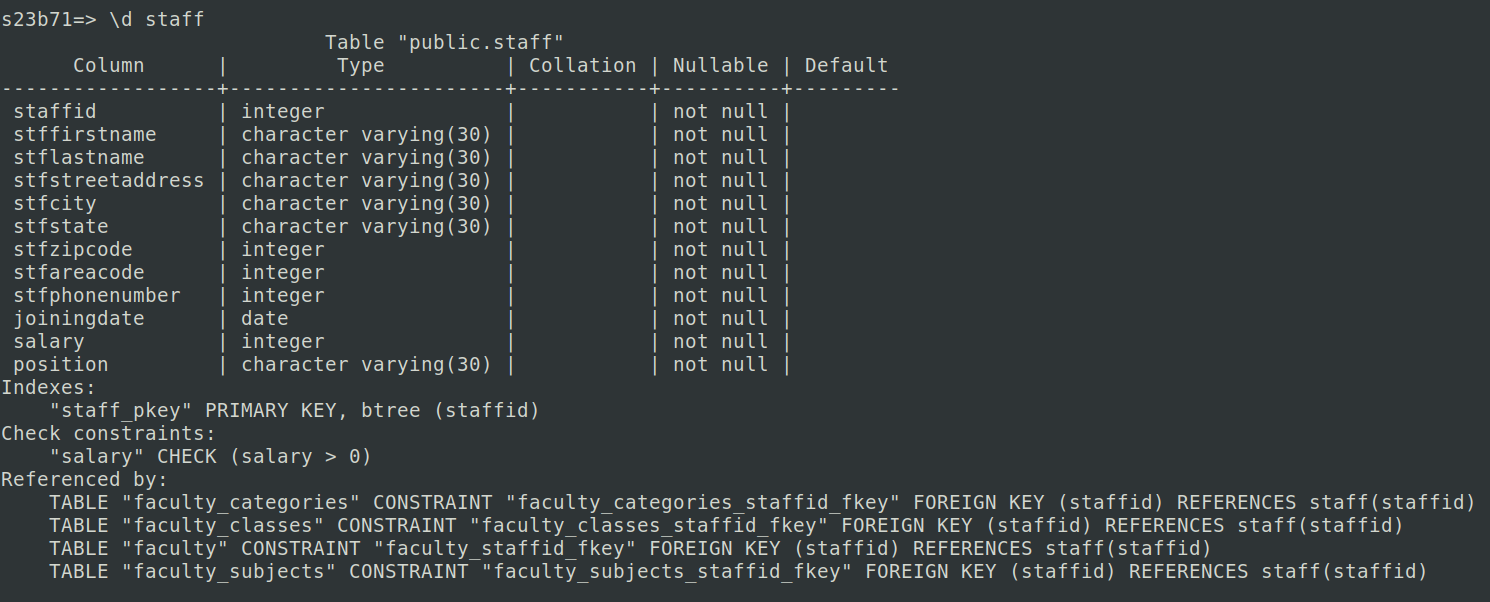
\includegraphics[width=\textwidth]{schema/staff.png}
\end{figure}

\subsubsection*{Faculty Table}
Query:
\begin{Verbatim}[frame=single,framerule=1pt,fontfamily=courier,fontsize=\small]
CREATE TABLE FACULTY(
StaffID INT PRIMARY KEY,
Title VARCHAR(30) NOT NULL,
Status VARCHAR(30) NOT NULL,
Tenured INT NOT NULL,
FOREIGN KEY (StaffID) REFERENCES STAFF(StaffID)
);
\end{Verbatim}
\begin{figure}[H]
    \centering
    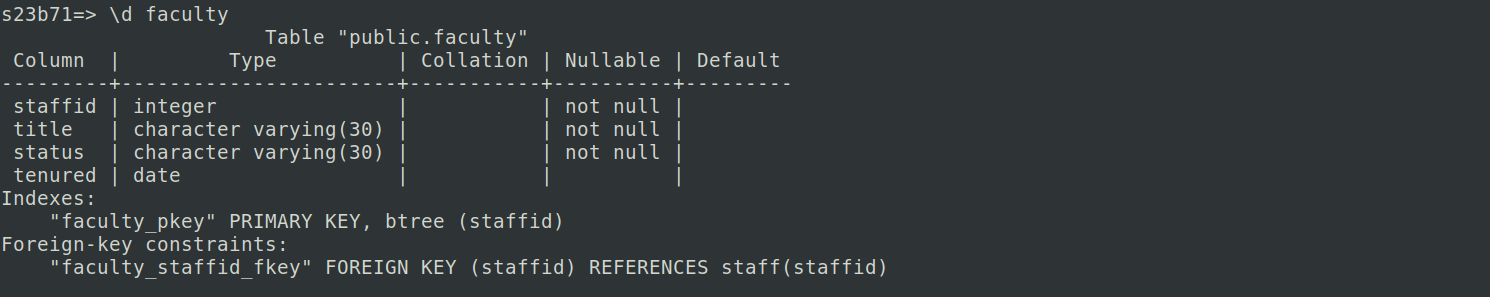
\includegraphics[width=\textwidth]{schema/faculty.png}
\end{figure}

\subsubsection*{Subjects Table}
Query:
\begin{Verbatim}[frame=single,framerule=1pt,fontfamily=courier,fontsize=\small]
CREATE TABLE SUBJECTS (
SubjectID INT PRIMARY KEY,
CategoryID INT,
SubjectCode INT NOT NULL,
SubjectName VARCHAR(30) NOT NULL,
SubjectDescription VARCHAR(30) NOT NULL,
FOREIGN KEY (CategoryID) REFERENCES CATEGORIES(CategoryID)
);
\end{Verbatim}
\begin{figure}[H]
    \centering
    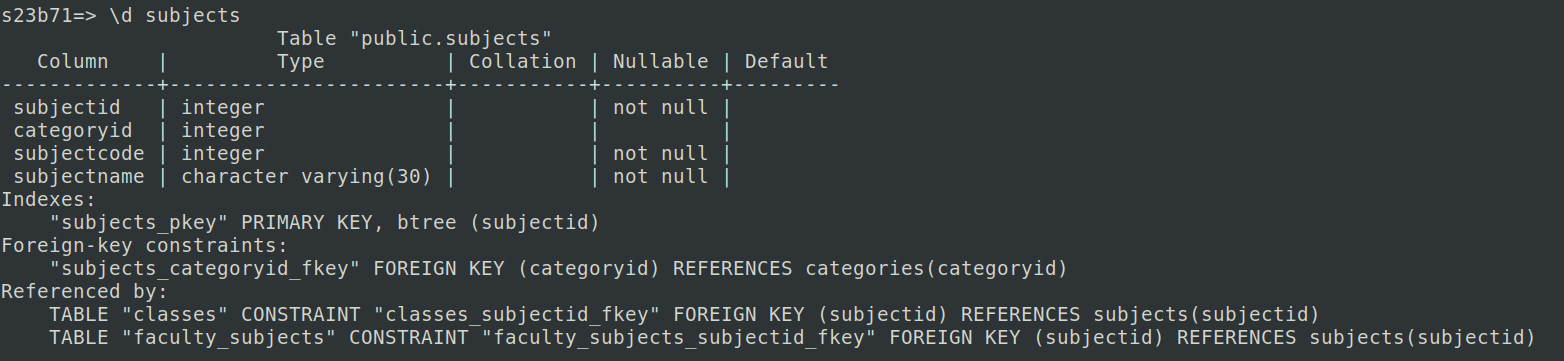
\includegraphics[width=\textwidth]{schema/subjects.png}
\end{figure}

\subsubsection*{Buildings Table}
Query:
\begin{Verbatim}[frame=single,framerule=1pt,fontfamily=courier,fontsize=\small]
CREATE TABLE BUILDINGS(
BuildingCode INT PRIMARY KEY,
BuildingName VARCHAR(30) NOT NULL,
NumberofFloors INT NOT NULL
);
\end{Verbatim}
\begin{figure}[H]
    \centering
    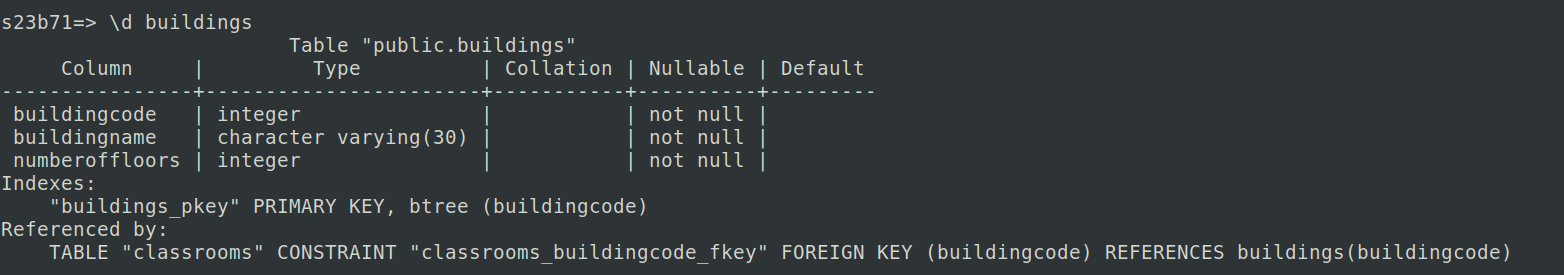
\includegraphics[width=\textwidth]{schema/buildings.png}
\end{figure}

\subsubsection*{Classrooms Table}
Query:
\begin{Verbatim}[frame=single,framerule=1pt,fontfamily=courier,fontsize=\small]
CREATE TABLE CLASSROOMS(
ClassRoomID INT PRIMARY KEY,
BuildingCode INT,
PhoneAvailable INT NOT NULL,
FOREIGN KEY (BuildingCode) REFERENCES BUILDINGS(BuildingCode)
);
\end{Verbatim}
\begin{figure}[H]
    \centering
    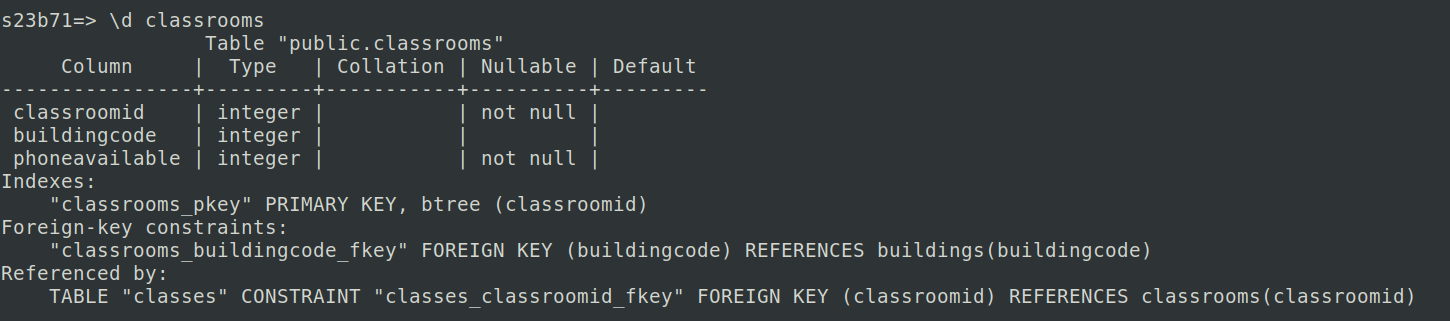
\includegraphics[width=\textwidth]{schema/classrooms.png}
\end{figure}

\subsubsection*{Classes Table}
Query:
\begin{Verbatim}[frame=single,framerule=1pt,fontfamily=courier,fontsize=\small]
CREATE TABLE CLASSES(
CLassID INT PRIMARY KEY,
SubjectID INT,
ClassRoomID INT,
StartTime TIME NOT NULL,
Duration INT NOT NULL,
FOREIGN KEY (SubjectID) REFERENCES SUBJECTS(SubjectID),
FOREIGN KEY (ClassRoomID) REFERENCES CLASSROOMS(ClassRoomID)
);
\end{Verbatim}
\begin{figure}[H]
    \centering
    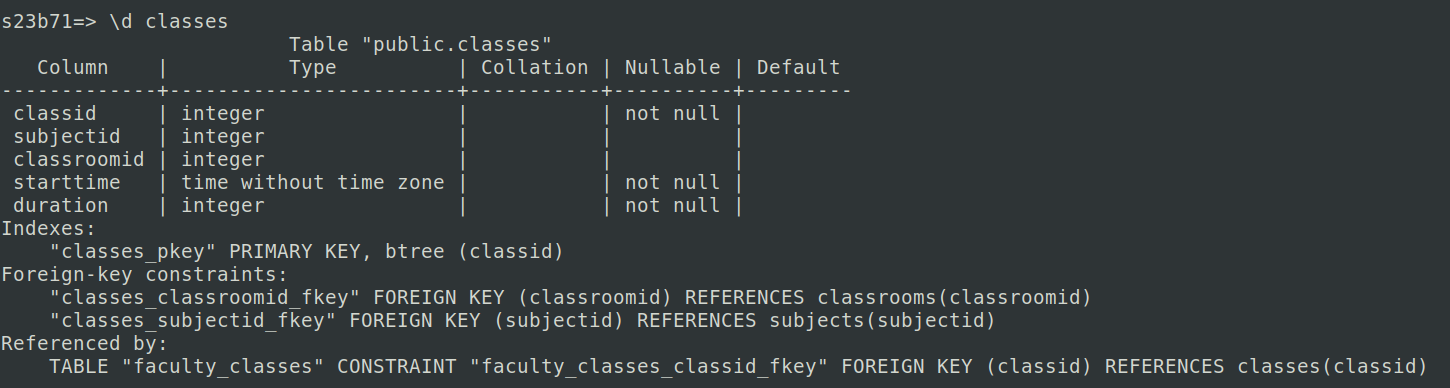
\includegraphics[width=\textwidth]{schema/classes.png}
\end{figure}

\subsubsection*{Categories Table}
Query:
\begin{Verbatim}[frame=single,framerule=1pt,fontfamily=courier,fontsize=\small]
CREATE TABLE CATEGORIES(
CategoryID INT PRIMARY KEY,
CategoryDescription VARCHAR(30) NOT NULL,
DepartmentID INT NOT NULL
);
\end{Verbatim}
\begin{figure}[H]
    \centering
    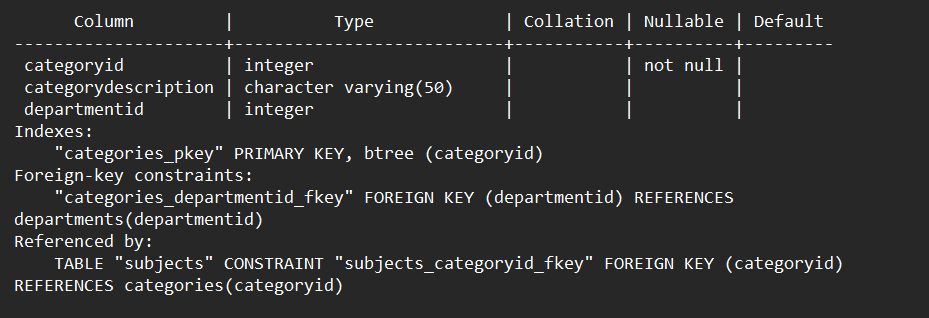
\includegraphics[width=\textwidth]{schema/categories.png}
\end{figure}

\subsubsection*{Faculty Subjects Table}
Query:
\begin{Verbatim}[frame=single,framerule=1pt,fontfamily=courier,fontsize=\small]
CREATE TABLE FACULTY_SUBJECTS(
StaffID INT ,
SubjectID INT,
ProficiencyRating INT NOT NULL,
PRIMARY KEY(StaffID,SubjectID),
FOREIGN KEY (StaffID) REFERENCES STAFF(StaffID),
FOREIGN KEY (SubjectID) REFERENCES SUBJECTS(SubjectID)
);
\end{Verbatim}
\begin{figure}[H]
    \centering
    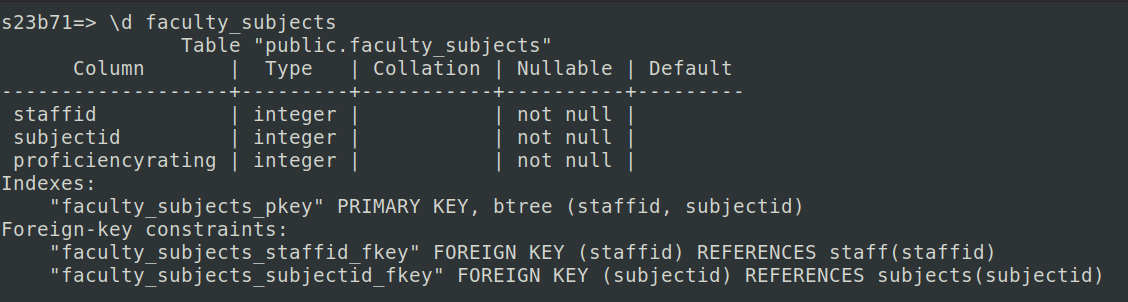
\includegraphics[width=\textwidth]{schema/faculty_subjects.png}
\end{figure}

\subsubsection*{Faculty Classes Table}
Query:
\begin{Verbatim}[frame=single,framerule=1pt,fontfamily=courier,fontsize=\small]
CREATE TABLE FACULTY_CLASSES(
StaffID INT ,
ClassID INT,
PRIMARY KEY(StaffID,ClassID),
FOREIGN KEY (StaffID) REFERENCES STAFF(StaffID),
FOREIGN KEY (ClassID) REFERENCES CLASSES(ClassID)
);
\end{Verbatim}
\begin{figure}[H]
    \centering
    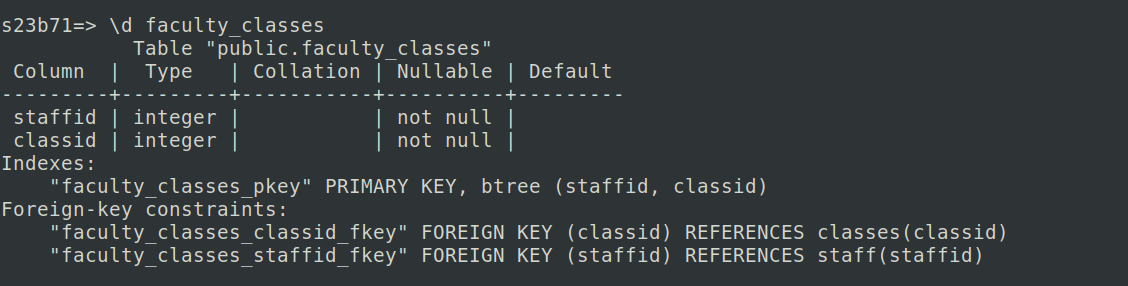
\includegraphics[width=\textwidth]{schema/faculty_classes.png}
\end{figure}

\subsubsection*{Students Table}
Query:
\begin{Verbatim}[frame=single,framerule=1pt,fontfamily=courier,fontsize=\small]
CREATE TABLE STUDENTS (
StudentID INT PRIMARY KEY,
StudFirstName VARCHAR(30) NOT NULL,
StudLastName VARCHAR(30) NOT NULL,
StudStreetAddress VARCHAR(30) NOT NULL,
StudCity VARCHAR(30) NOT NULL,
StudState VARCHAR(30) NOT NULL,
StudZipCode INT NOT NULL,
StudAreaCode INT NOT NULL,
StudPhoneNumber INT NOT NULL
);
\end{Verbatim}
\begin{figure}[H]
    \centering
    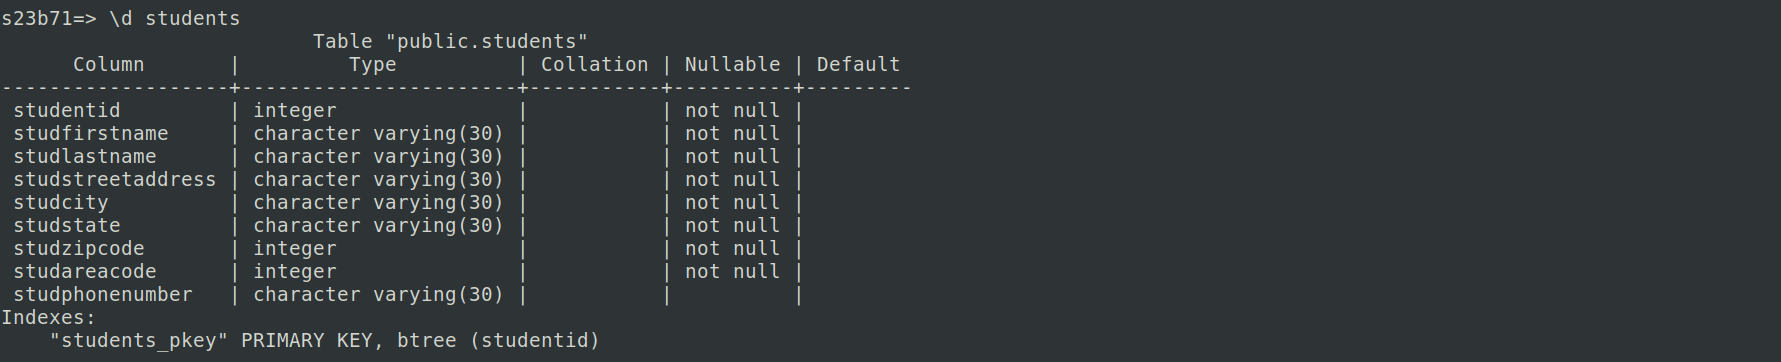
\includegraphics[width=\textwidth]{schema/students.png}
\end{figure}

\subsubsection*{Student Class Status Table}
Query:
\begin{Verbatim}[frame=single,framerule=1pt,fontfamily=courier,fontsize=\small]
CREATE TABLE STUDENT_CLASS_STATUS (
ClassStatus INT PRIMARY KEY,
ClassDescription VARCHAR(30) NOT NULL
);
\end{Verbatim}
\begin{figure}[H]
    \centering
    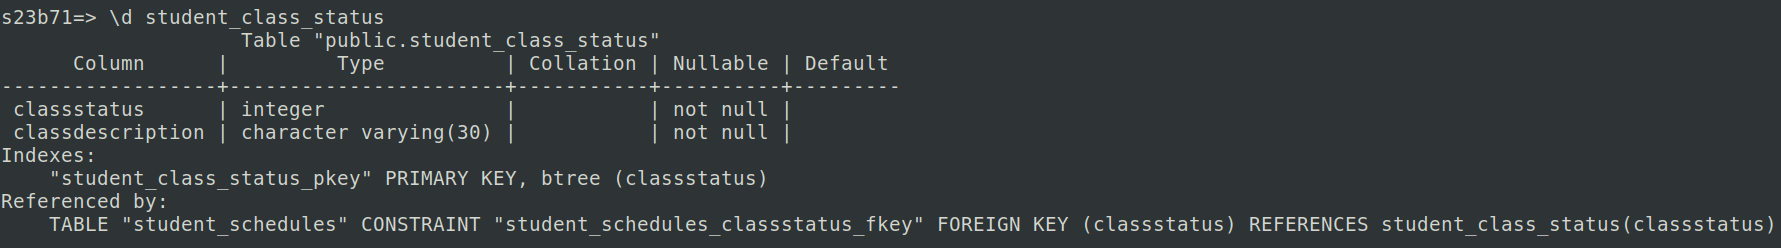
\includegraphics[width=\textwidth]{schema/student_class_status.png}
\end{figure}

\subsubsection*{Student Schedules Table}
Query:
\begin{Verbatim}[frame=single,framerule=1pt,fontfamily=courier,fontsize=\small]
CREATE TABLE STUDENT_SCHEDULES (
ClassID INT,
StudentID INT,
ClassStatus INT,
Grade VARCHAR(30) NOT NULL,
PRIMARY KEY(ClassID,StudentID),
FOREIGN KEY (ClassStatus) REFERENCES STUDENT_CLASS_STATUS(ClassStatus)
);
\end{Verbatim}
\begin{figure}[H]
    \centering
    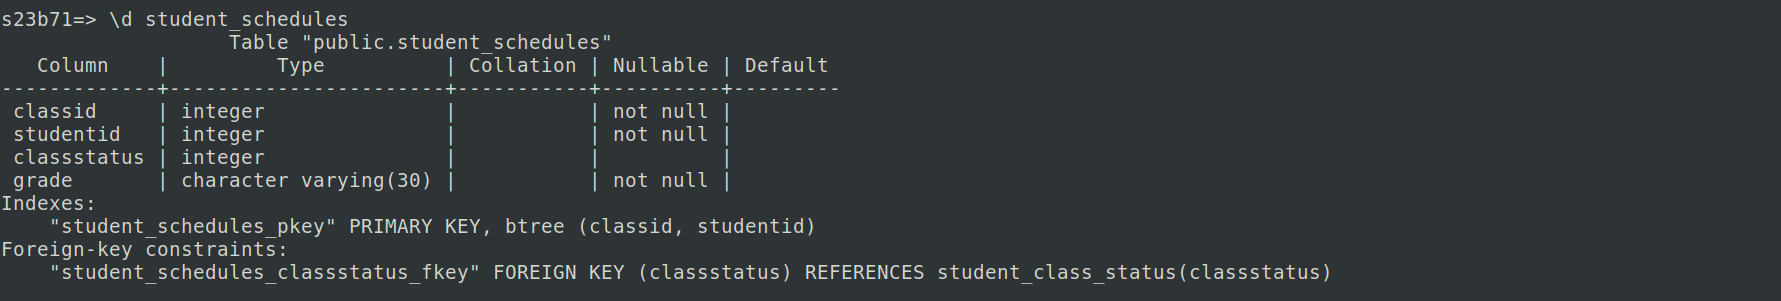
\includegraphics[width=\textwidth]{schema/student_schedules.png}
\end{figure}

\subsection*{3. Write commands to}
\subsubsection* {a. Create and execute an alter table command to rename column 'DateHired' from Staff table to 'JoiningDate'.}
Query:
\begin{Verbatim}[frame=single,framerule=1pt,fontfamily=courier,fontsize=\small]
ALTER TABLE STAFF RENAME COLUMN DateHired TO JoiningDate;
\end{Verbatim}
\begin{figure}[H]
    \centering
    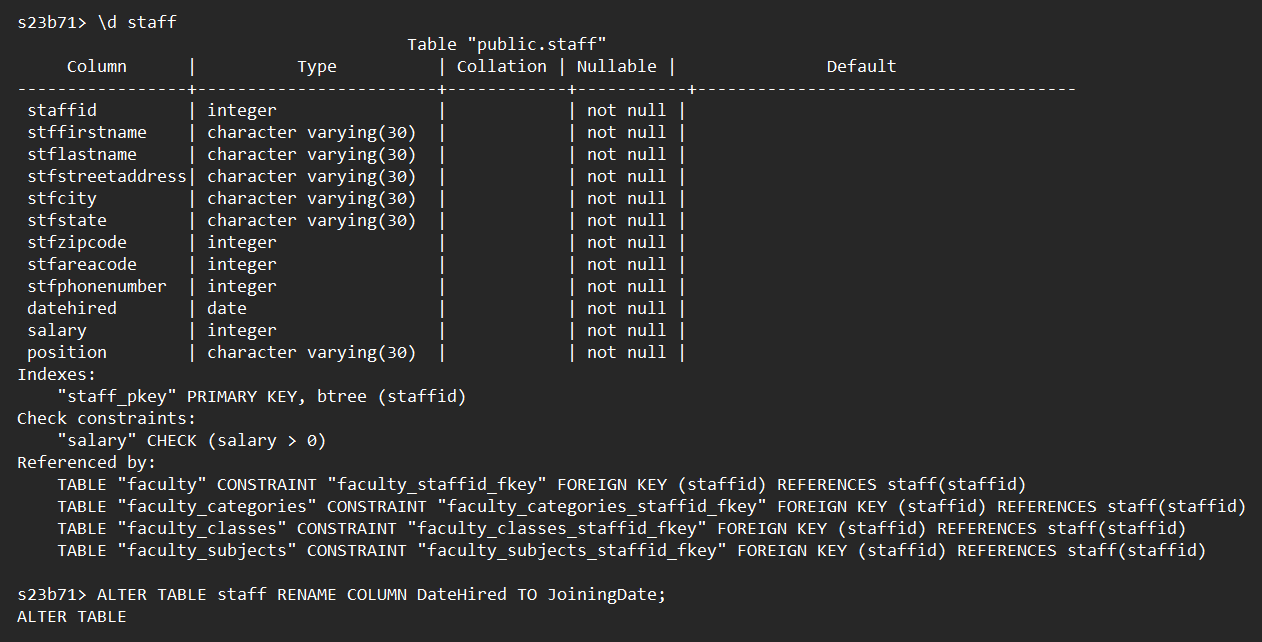
\includegraphics[width=\textwidth]{cycle1/1.3.1.png}
    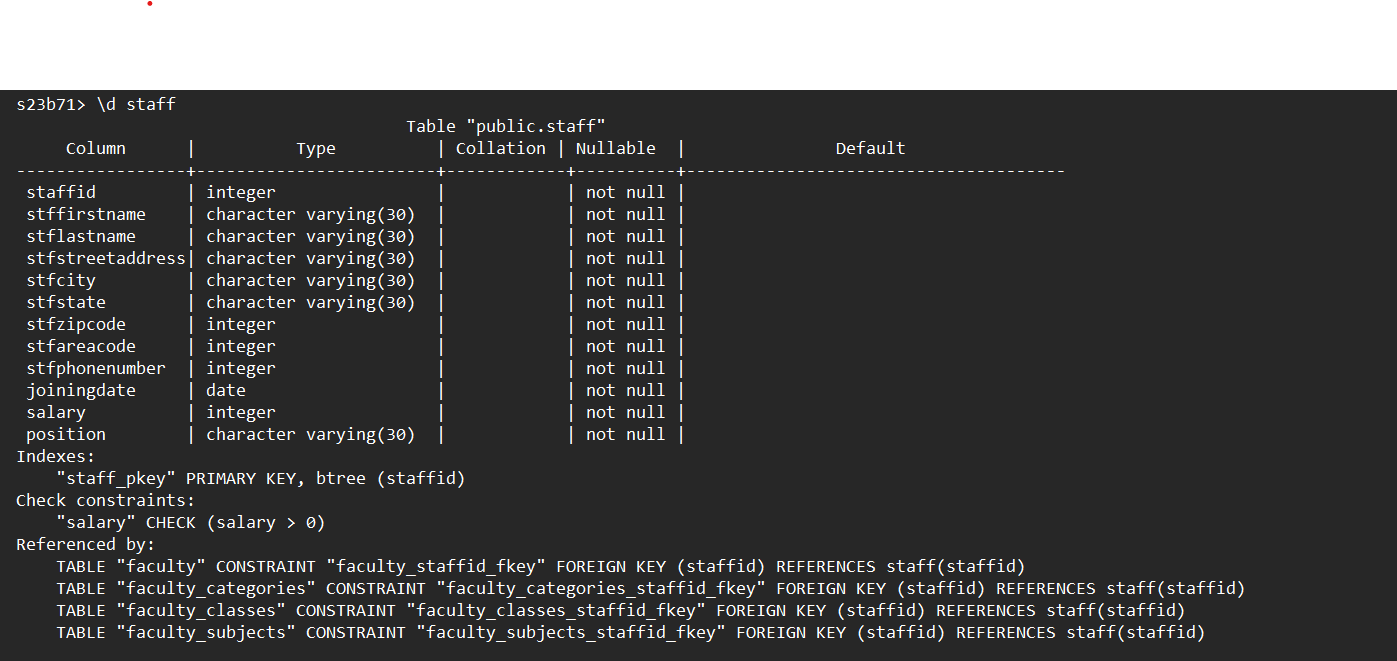
\includegraphics[width=\textwidth]{cycle1/1.3.2.png}
\end{figure}

\subsubsection* {b . Create and execute an alter table command to remove the column 'SubjectDescription' from the Subjects table.}
Query:
\begin{Verbatim}[frame=single,framerule=1pt,fontfamily=courier,fontsize=\small]
ALTER TABLE SUBJECTS DROP COLUMN SubjectDescription;
\end{Verbatim}
\begin{figure}[H]
    \centering
    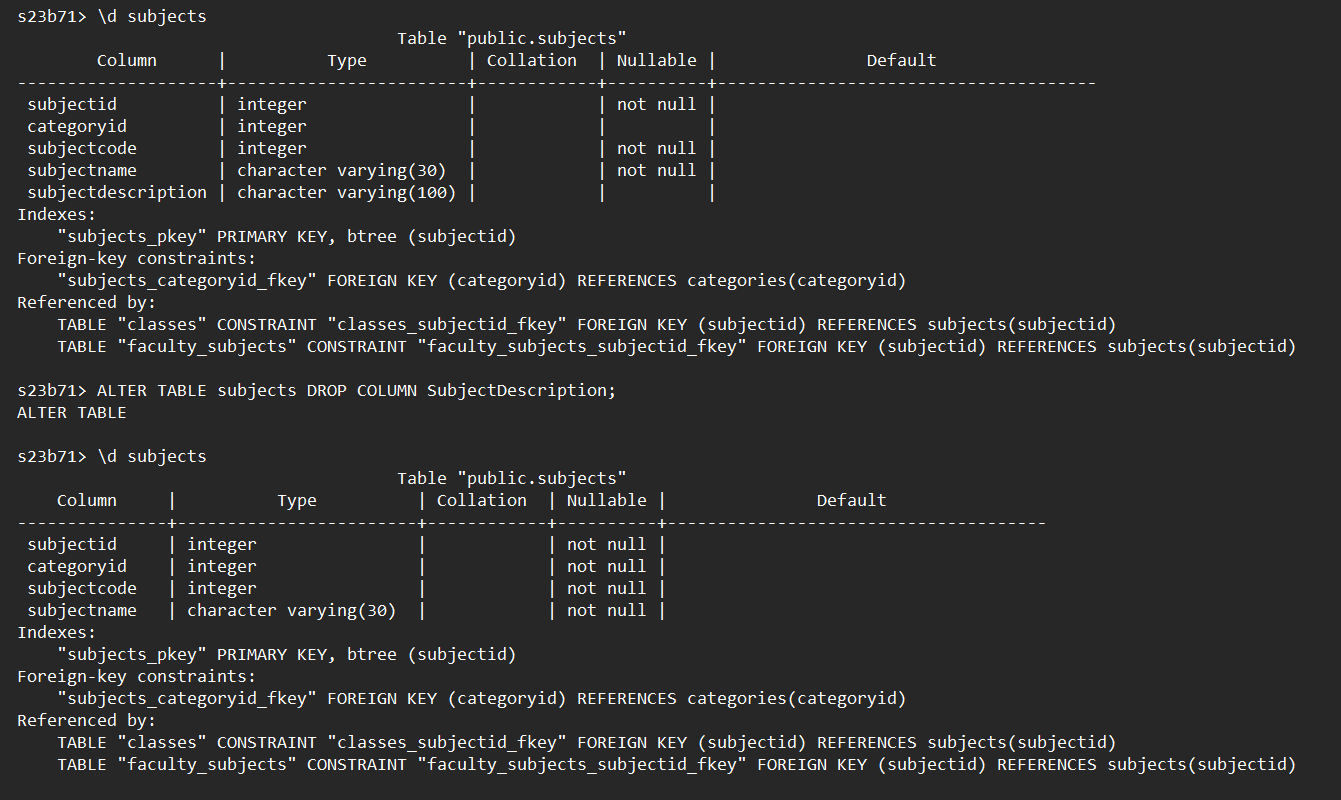
\includegraphics[width=\textwidth]{cycle1/1.3.3.png}
\end{figure}

\subsection*{Result}
Query executed and output obtained successfully.

\newpage
\section*{\centering{Cycle 2}}

\subsection*{1. Insert data in the created database.}
Query:
% Insert into BUILDINGS table
\begin{Verbatim}[frame=single,framerule=1pt,fontfamily=courier,fontsize=\small]
INSERT INTO buildings (buildingcode, buildingname, numberoffloors) VALUES 
(1, 'Building A', 3),
(2, 'Building B', 4),
(3, 'Building C', 2),
(4, 'Building D', 3),
(5, 'Building E', 1);
\end{Verbatim}
\begin{figure}[H]
    \centering
    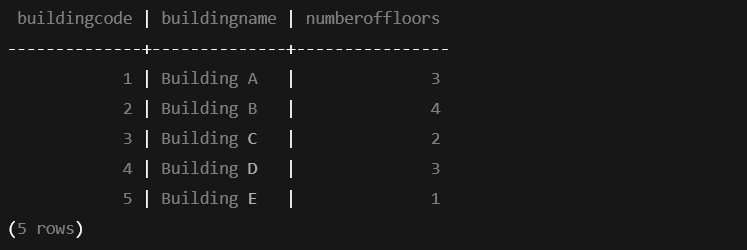
\includegraphics[width=\textwidth]{select/buildings.png}
\end{figure}

% Insert into CATEGORIES table
\begin{Verbatim}[frame=single,framerule=1pt,fontfamily=courier,fontsize=\small]
INSERT INTO categories (categoryid, categorydescription, departmentid) VALUES 
(1, 'Math', 1),
(2, 'Science', 2),
(3, 'Arts', 3),
(4, 'History', 4),
(5, 'Literature', 5);
\end{Verbatim}
\begin{figure}[H]
    \centering
    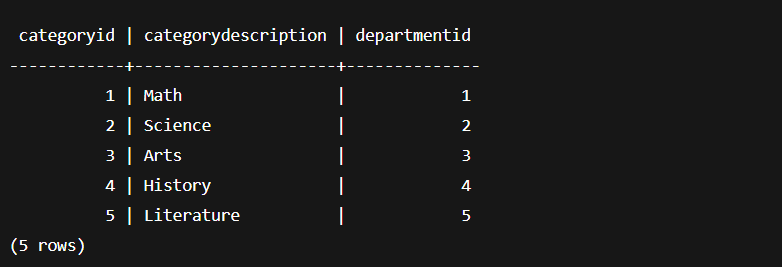
\includegraphics[width=\textwidth]{select/categories.png}
\end{figure}

% Insert into CLASSES table
\begin{Verbatim}[frame=single,framerule=1pt,fontfamily=courier,fontsize=\small]
INSERT INTO classes (classid, subjectid, classroomid, starttime, duration) VALUES 
(1, 1, 1, '09:00:00', 60),
(2, 2, 2, '10:30:00', 75),
(3, 3, 3, '14:00:00', 30),
(4, 4, 4, '08:00:00', 120),
(5, 5, 5, '16:30:00', 20);
\end{Verbatim}
\begin{figure}[H]
    \centering
    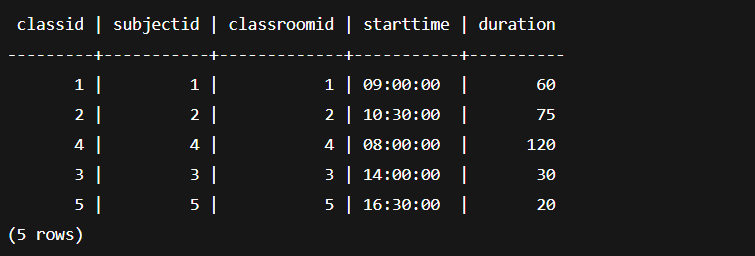
\includegraphics[width=\textwidth]{select/classes.png}
\end{figure}

% Insert into CLASSROOMS table
\begin{Verbatim}[frame=single,framerule=1pt,fontfamily=courier,fontsize=\small]
INSERT INTO classrooms (classroomid, buildingcode, phoneavailable) VALUES 
(1, 1, 1),
(2, 2, 0),
(3, 3, 1),
(4, 4, 0),
(5, 5, 1);
\end{Verbatim}
\begin{figure}[H]
    \centering
    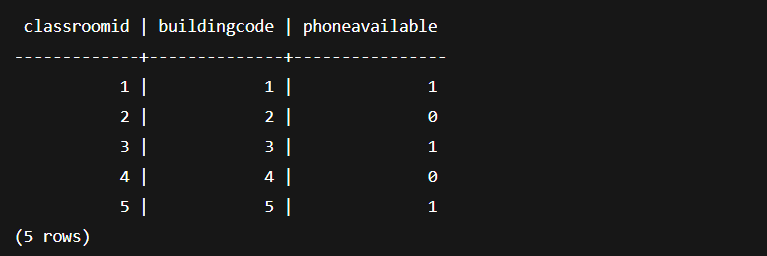
\includegraphics[width=\textwidth]{select/classrooms.png}
\end{figure}

% Insert into STAFF table
\begin{Verbatim}[frame=single,framerule=1pt,fontfamily=courier,fontsize=\small]
INSERT INTO staff (staffid, stffirstname, stflastname, stfstreetaddress, 
    stfcity, stfstate, stfzipcode, stfareacode, stfphonenumber, joiningdate, 
    salary, "position") VALUES 
(1, 'John', 'Doe', '123 Elm St', 'Springfield', 'IL', 62701, 217, 5551234, 
    '2020-01-01', 50000, 'Professor'),
(2, 'Jane', 'Smith', '456 Oak St', 'Champaign', 'IL', 61820, 217, 5555678, 
    '2019-03-15', 55000, 'Lecturer'),
(3, 'Mike', 'Johnson', '789 Pine St', 'Peoria', 'IL', 61602, 309, 5558765, 
    '2021-08-22', 60000, 'Associate Professor'),
(4, 'Emily', 'Davis', '101 Maple St', 'Bloomington', 'IL', 61701, 309, 5552345, 
    '2022-11-05', 52000, 'Assistant Professor'),
(5, 'Sarah', 'Brown', '202 Birch St', 'Decatur', 'IL', 62521, 217, 5556789, 
    '2023-02-28', 48000, 'Instructor');
\end{Verbatim}
\begin{figure}[H]
    \centering
    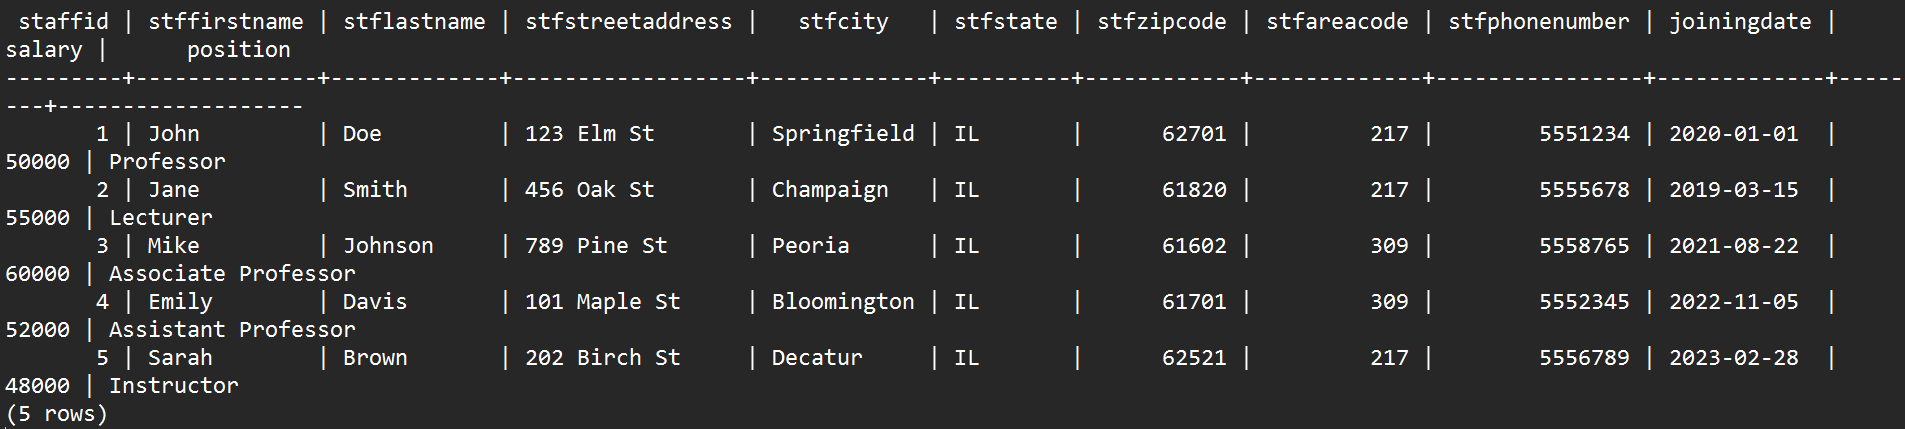
\includegraphics[width=\textwidth]{select/staff.png}
\end{figure}

% Insert into FACULTY table
\begin{Verbatim}[frame=single,framerule=1pt,fontfamily=courier,fontsize=\small]
INSERT INTO faculty (staffid, title, status, tenured) VALUES 
(1, 'Dr.', 'Active', '2030-06-06'),
(2, 'Prof.', 'Active', '2026-08-09'),
(3, 'Dr.', 'On Leave', '2032-01-01'),
(4, 'Dr.', 'Active', '2025-08-08'),
(5, 'Prof.', 'Retired', '2028-02-01');
\end{Verbatim}
\begin{figure}[H]
    \centering
    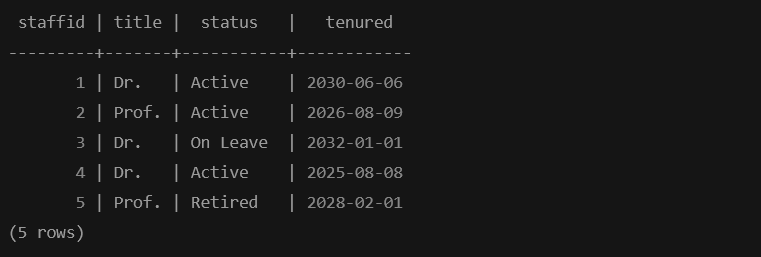
\includegraphics[width=\textwidth]{select/faculty.png}
\end{figure}

% Insert into FACULTY_CATEGORIES table
\begin{Verbatim}[frame=single,framerule=1pt,fontfamily=courier,fontsize=\small]
INSERT INTO faculty_categories (staffid, categoryid) VALUES 
(1, 1),
(2, 2),
(3, 3),
(4, 4),
(5, 5);
\end{Verbatim}
\begin{figure}[H]
    \centering
    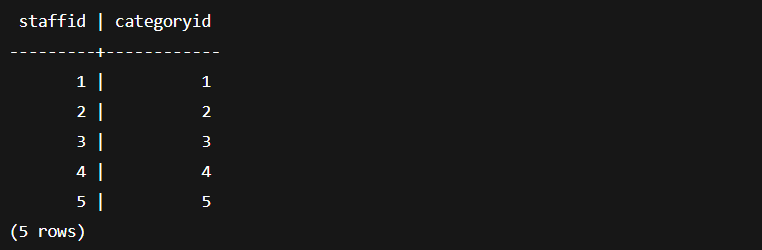
\includegraphics[width=\textwidth]{select/faculty_categories.png}
\end{figure}

% Insert into FACULTY_CLASSES table
\begin{Verbatim}[frame=single,framerule=1pt,fontfamily=courier,fontsize=\small]
INSERT INTO faculty_classes (staffid, classid) VALUES 
(1, 1),
(2, 2),
(3, 3),
(4, 4),
(5, 5);
\end{Verbatim}
\begin{figure}[H]
    \centering
    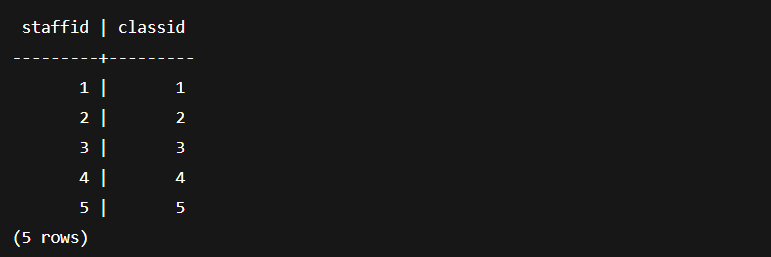
\includegraphics[width=\textwidth]{select/faculty_classes.png}
\end{figure}

% Insert into FACULTY_SUBJECTS table
\begin{Verbatim}[frame=single,framerule=1pt,fontfamily=courier,fontsize=\small]
INSERT INTO faculty_subjects (staffid, subjectid, proficiencyrating) VALUES 
(1, 1, 5),
(2, 2, 4),
(4, 4, 4),
(1, 3, 5),
(2, 5, 3);
\end{Verbatim}
\begin{figure}[H]
    \centering
    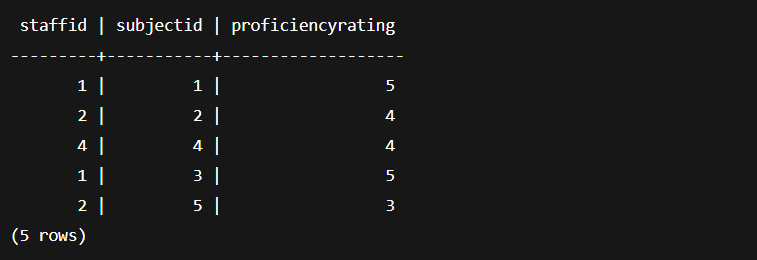
\includegraphics[width=\textwidth]{select/faculty_subjects.png}
\end{figure}

% Insert into STUDENTS table
\begin{Verbatim}[frame=single,framerule=1pt,fontfamily=courier,fontsize=\small]
INSERT INTO students (studentid, studfirstname, studlastname, 
    studstreetaddress, studcity, studstate, studzipcode, studareacode, 
    studphonenumber) VALUES 
(1, 'Alice', 'Green', '100 Oak St', 'Chicago', 'IL', 60601, 312, '9512334466'),
(2, 'Bob', 'White', '200 Pine St', 'Naperville', 'IL', 60540, 630, '9534657562'),
(3, 'Charlie', 'Black', '300 Birch St', 'Aurora', 'IL', 60502, 630, '1234343556'),
(4, 'David', 'Blue', '400 Maple St', 'Peoria', 'IL', 61604, 309, '1234453434'),
(5, 'Eva', 'Red', '500 Elm St', 'Rockford', 'IL', 61101, 815, '9598943580');
\end{Verbatim}
\begin{figure}[H]
    \centering
    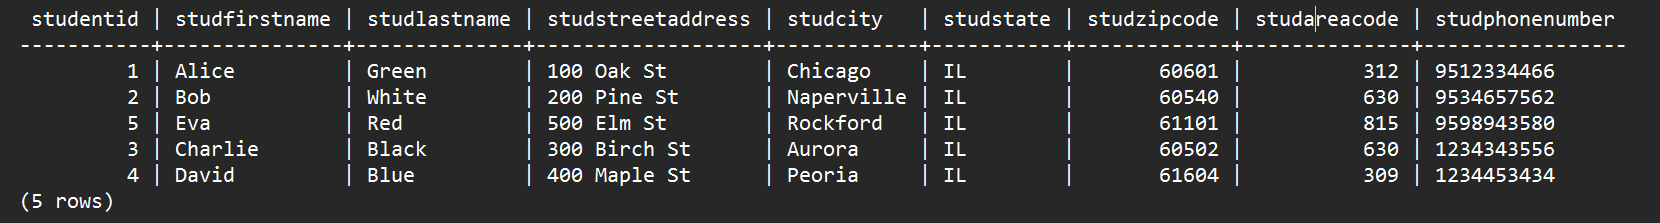
\includegraphics[width=\textwidth]{select/student.png}
\end{figure}

% Insert into STUDENT_CLASS_STATUS table
\begin{Verbatim}[frame=single,framerule=1pt,fontfamily=courier,fontsize=\small]
INSERT INTO student_class_status (classstatus, classdescription) VALUES 
(1, 'Enrolled'),
(2, 'Completed'),
(3, 'Dropped'),
(4, 'Failed'),
(5, 'Withdrawn');
\end{Verbatim}
\begin{figure}[H]
    \centering
    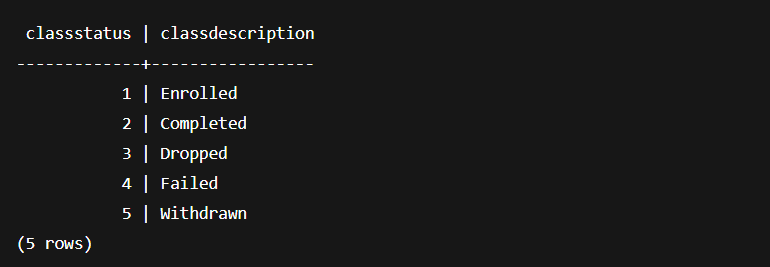
\includegraphics[width=\textwidth]{select/student_class_status.png}
\end{figure}

% Insert into STUDENT_SCHEDULES table
\begin{Verbatim}[frame=single,framerule=1pt,fontfamily=courier,fontsize=\small]
INSERT INTO student_schedules (classid, studentid, classstatus, grade) VALUES 
(1, 1, 1, 'A'),
(1, 2, 2, 'B'),
(1, 3, 3, 'C'),
(2, 4, 4, 'D'),
(2, 5, 5, 'F');
\end{Verbatim}
\begin{figure}[H]
    \centering
    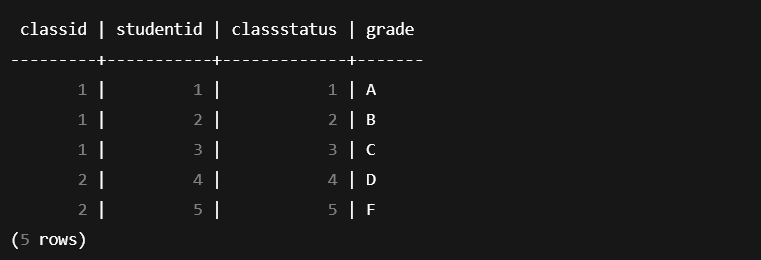
\includegraphics[width=\textwidth]{select/student_schedules.png}
\end{figure}

% Insert into SUBJECTS table
\begin{Verbatim}[frame=single,framerule=1pt,fontfamily=courier,fontsize=\small]
INSERT INTO subjects (subjectid, categoryid, subjectcode, subjectname) VALUES 
(1, 1, 101, 'Calculus I'),
(2, 2, 201, 'Introduction to Programming'),
(3, 3, 301, 'Classical Mechanics'),
(4, 4, 401, 'Cell Biology'),
(5, 5, 501, 'Organic Chemistry');
\end{Verbatim}
\begin{figure}[H]
    \centering
    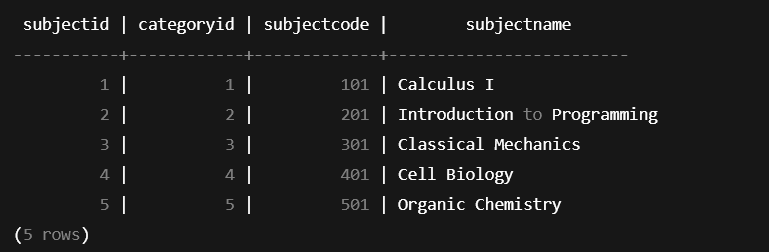
\includegraphics[width=\textwidth]{select/subjects.png}
\end{figure}

\subsection*{2. Display the list of faculties who have more than 5 year tenure period.}
Query:
\begin{Verbatim}[frame=single,framerule=1pt,fontfamily=courier,fontsize=\small]
SELECT * FROM faculty f,staff s WHERE f.staffid = s.staffid 
and (f.tenured - s.joiningdate)/365 > 5;
\end{Verbatim}
\begin{figure}[H]
    \centering
    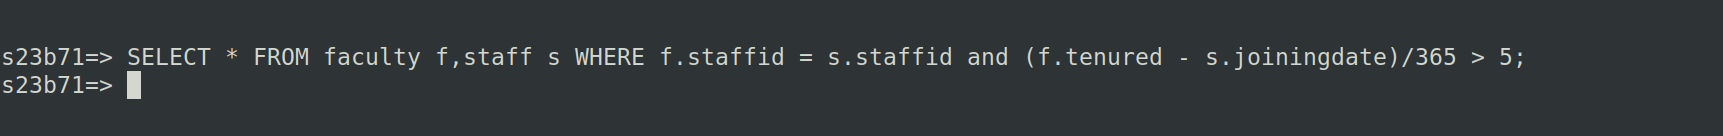
\includegraphics[width=\textwidth]{cycle2/2.2.1.png}
\end{figure}
\begin{figure}[H]
    \centering
    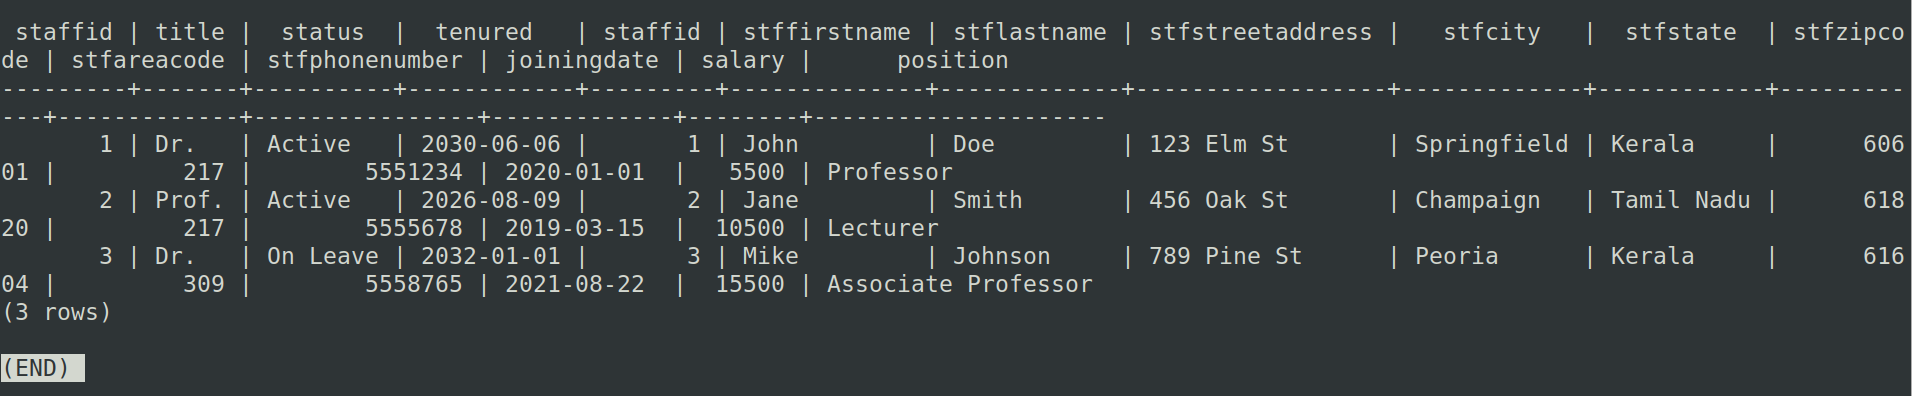
\includegraphics[width=\textwidth]{cycle2/2.2.2.png}
\end{figure}

\subsection*{3. Calculate the remaining tenure period from the current date.}
Query:
\begin{Verbatim}[frame=single,framerule=1pt,fontfamily=courier,fontsize=\small]
SELECT *,(tenured - CURRENT_DATE)/365 as "Remaining Years" FROM faculty;
\end{Verbatim}
\begin{figure}[H]
    \centering
    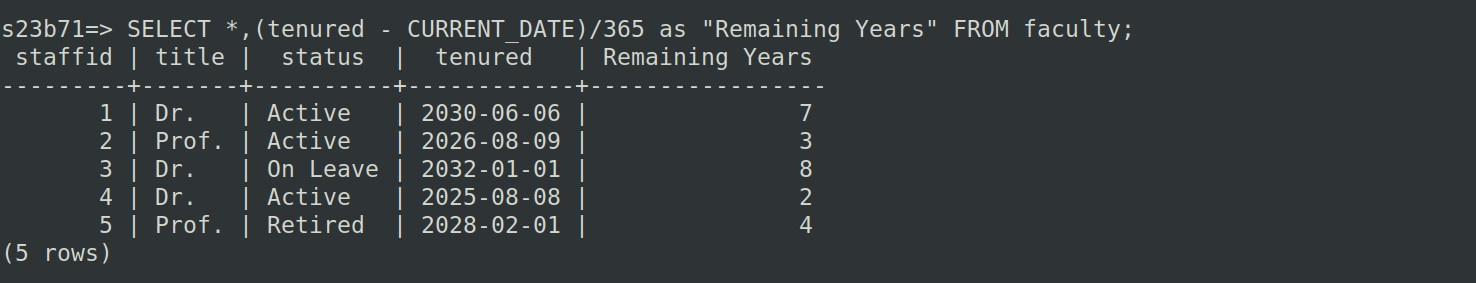
\includegraphics[width=\textwidth]{cycle2/2.3.png}
\end{figure}

\subsection*{4. Display the list of staff who have salary greater than 10000 and less than 50000.}
Query:
\begin{Verbatim}[frame=single,framerule=1pt,fontfamily=courier,fontsize=\small]
SELECT * FROM staff WHERE salary > 10000 and salary < 50000;
\end{Verbatim}
\begin{figure}[H]
    \centering
    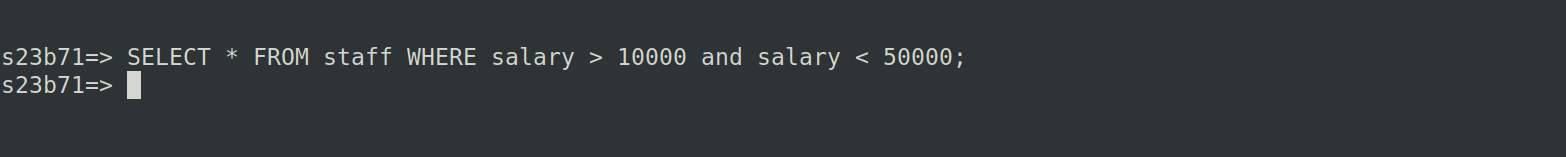
\includegraphics[width=\textwidth]{cycle2/2.4.1.png}
\end{figure}
\begin{figure}[H]
    \centering
    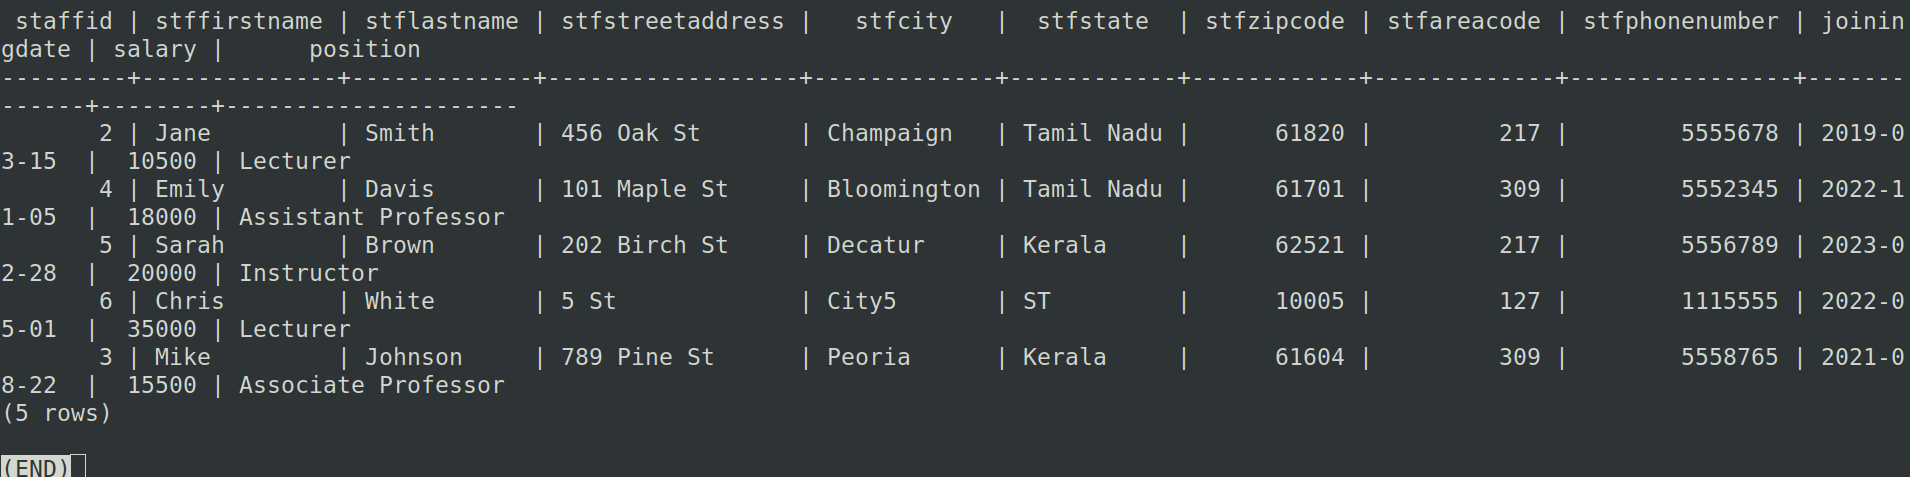
\includegraphics[width=\textwidth]{cycle2/2.4.2.png}
\end{figure}

\subsection*{5. Count the no: of positions in the staff relation.}
Query:
\begin{Verbatim}[frame=single,framerule=1pt,fontfamily=courier,fontsize=\small]
SELECT COUNT(DISTINCT position) FROM staff;
\end{Verbatim}
\begin{figure}[H]
    \centering
    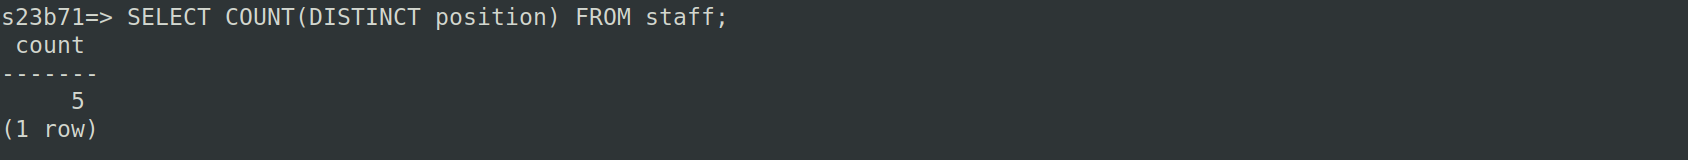
\includegraphics[width=\textwidth]{cycle2/2.5.png}
\end{figure}

\subsection*{6. Count the no: of staff from a particular area code.}
Query:
\begin{Verbatim}[frame=single,framerule=1pt,fontfamily=courier,fontsize=\small]
SELECT COUNT(*) FROM staff WHERE stfareacode = 217;
\end{Verbatim}
\begin{figure}[H]
    \centering
    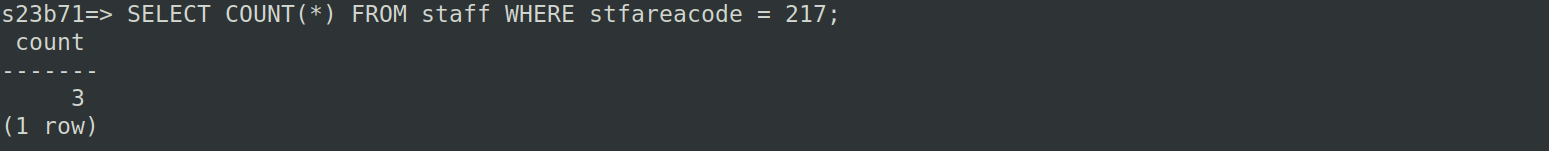
\includegraphics[width=\textwidth]{cycle2/2.6.png}
\end{figure}

\subsection*{Result}
Query executed and output obtained successfully.

\newpage
\section*{\centering{Cycle 3}}

\subsection*{1. Display the count of teachers teaching either two or three different subjects}
Query:
\begin{Verbatim}[frame=single,framerule=1pt,fontfamily=courier,fontsize=\small]
SELECT staffid,COUNT(subjectid) FROM faculty_subjects 
GROUP BY staffid HAVING COUNT(subjectid) IN (2,3);
\end{Verbatim}
\begin{figure}[H]
    \centering
    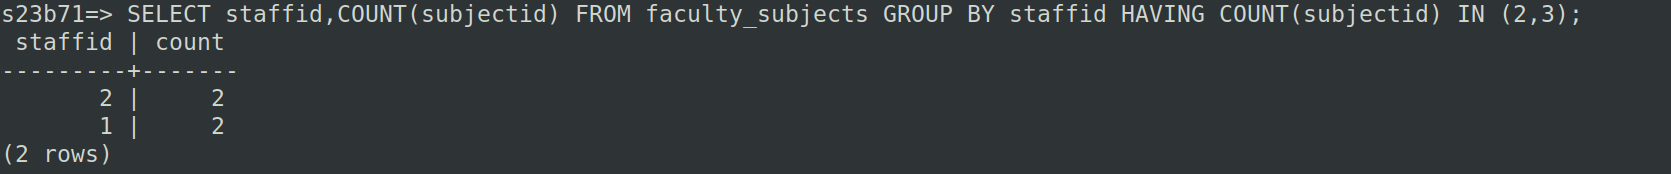
\includegraphics[width=\textwidth]{cycle3/3.1.png}
\end{figure}

\subsection*{2. Display the maximum of average salary from Staff table based on their positions}
Query:
\begin{Verbatim}[frame=single,framerule=1pt,fontfamily=courier,fontsize=\small]
SELECT MAX(Average) AS "MAXIMUM SALARY" FROM 
(SELECT AVG(Salary) as Average FROM STAFF GROUP BY position) 
AS "MAXIMUM SALARY";
\end{Verbatim}
\begin{figure}[H]
    \centering
    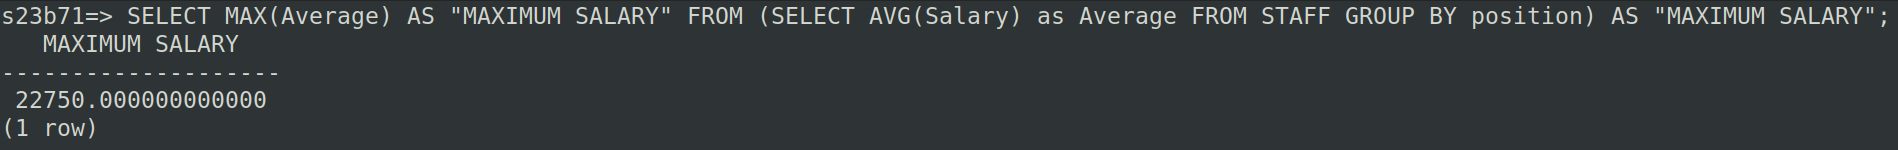
\includegraphics[width=\textwidth]{cycle3/3.2.png}
\end{figure}

\subsection*{3. Display the minimum grade of students for each subject from each class}
Query:
\begin{Verbatim}[frame=single,framerule=1pt,fontfamily=courier,fontsize=\small]
SELECT classid,MAX(grade) AS "Min Grade" FROM student_schedules 
GROUP BY classid ORDER BY classid;
\end{Verbatim}
\begin{figure}[H]
    \centering
    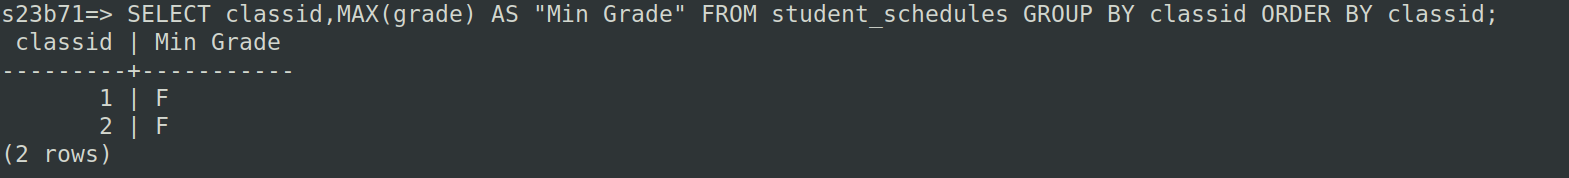
\includegraphics[width=\textwidth]{cycle3/3.3.png}
\end{figure}

\subsection*{4. Display subject name which contains character 'a'}
Query:
\begin{Verbatim}[frame=single,framerule=1pt,fontfamily=courier,fontsize=\small]
SELECT subjectname AS Subject FROM subjects WHERE subjectname LIKE '%a%';
\end{Verbatim}
\begin{figure}[H]
    \centering
    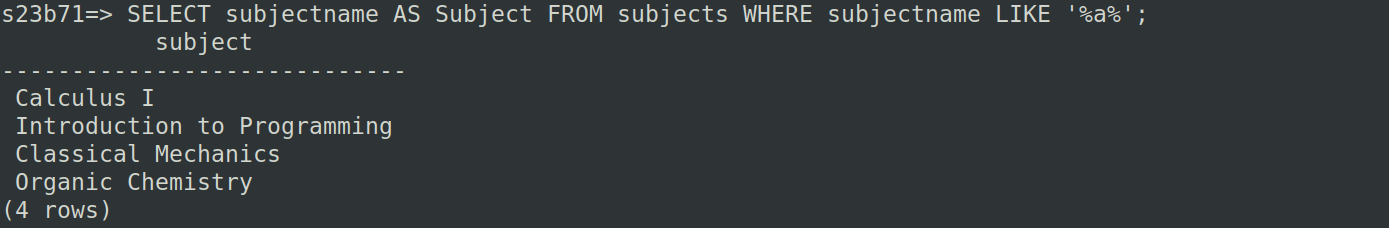
\includegraphics[width=\textwidth]{cycle3/3.4.png}
\end{figure}

\subsection*{5. Display the name of students having mobile no starting with '95'}
Query:
\begin{Verbatim}[frame=single,framerule=1pt,fontfamily=courier,fontsize=\small]
SELECT studphonenumber AS "Phone Number" FROM students 
WHERE studphonenumber LIKE '95%';
\end{Verbatim}
\begin{figure}[H]
    \centering
    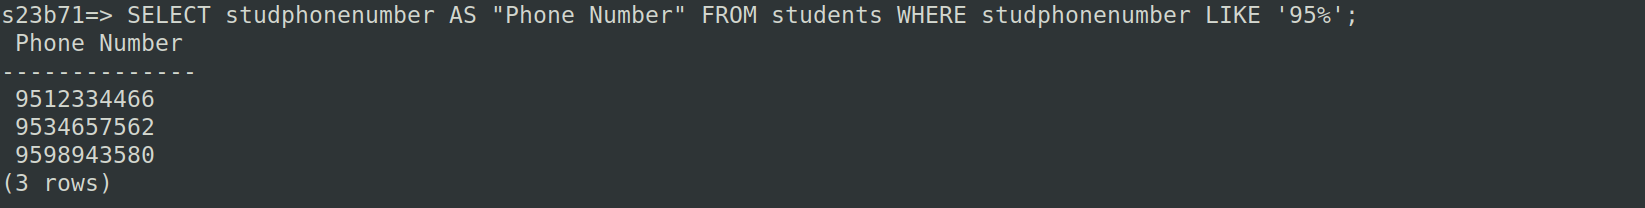
\includegraphics[width=\textwidth]{cycle3/3.5.png}
\end{figure}

\subsection*{6. Retrieve Class ID and maximum duration available in Classes where maximum duration is less than 45 minutes}
Query:
\begin{Verbatim}[frame=single,framerule=1pt,fontfamily=courier,fontsize=\small]
SELECT classid AS "Class ID",MAX(duration) FROM classes 
GROUP BY classid ORDER BY classid;
\end{Verbatim}
\begin{figure}[H]
    \centering
    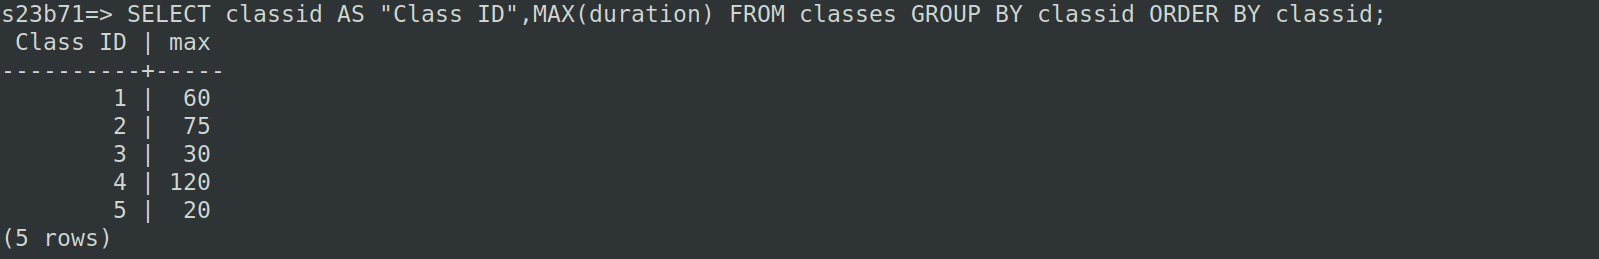
\includegraphics[width=\textwidth]{cycle3/3.6.png}
\end{figure}

\subsection*{7. Display the list of students based on Student ID in ascending order and Student Name in descending order, Group by Subject Name}
Query:
\begin{Verbatim}[frame=single,framerule=1pt,fontfamily=courier,fontsize=\small]
SELECT st.studentid,st.studfirstname,st.studlastname,su.subjectname 
FROM students st, student_schedules ss, classes cl,subjects su  
WHERE st.studentid = ss.studentid AND ss.classid = cl.classid 
AND cl.subjectid = su.subjectid GROUP BY st.studfirstname,
st.studentid,su.subjectname ORDER BY st.studentid ASC;
\end{Verbatim}
\begin{figure}[H]
    \centering
    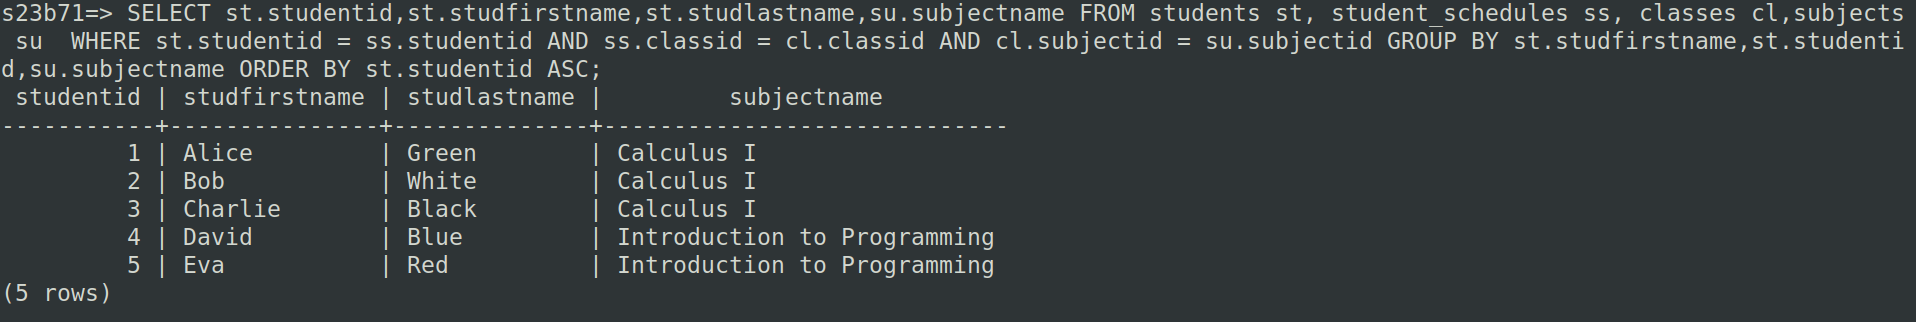
\includegraphics[width=\textwidth]{cycle3/3.7.png}
\end{figure}

\subsection*{8. Display position and average salary of staff belonging to state "Kerala" or "Tamil Nadu" where salary is more than 10000 and average salary is less than 25000}
Query:
\begin{Verbatim}[frame=single,framerule=1pt,fontfamily=courier,fontsize=\small]
SELECT position,AVG(salary) FROM staff WHERE salary > 10000 
AND stfstate IN ('Kerala','Tamil Nadu') GROUP BY position 
HAVING AVG(salary) < 25000;
\end{Verbatim}
\begin{figure}[H]
    \centering
    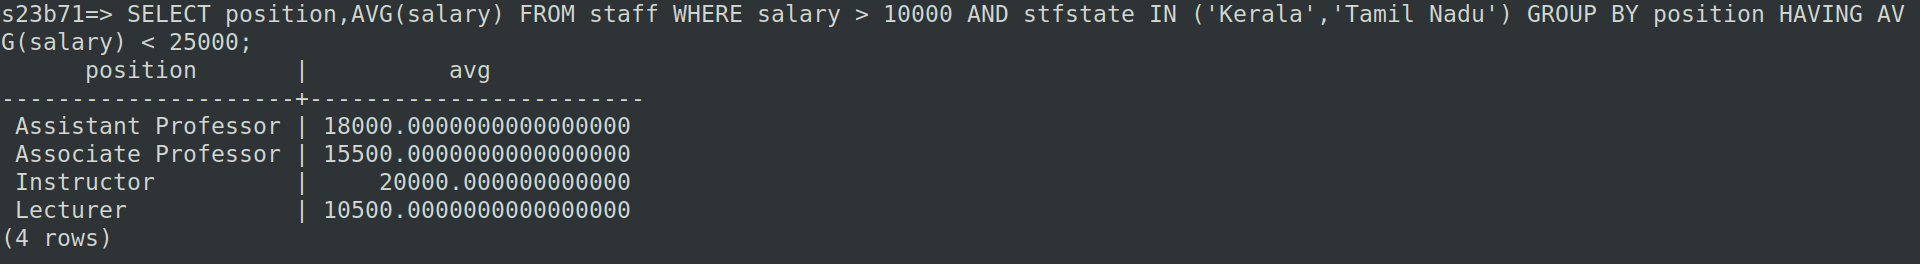
\includegraphics[width=\textwidth]{cycle3/3.8.png}
\end{figure}

\subsection*{Result}
Query executed and output obtained successfully.

\newpage
\section*{\centering{Cycle 4}}

\subsection*{1.a. Revoke insert privilege for a user on table Students and check whether you are able to insert a row in to the table}
Query:
\begin{Verbatim}[frame=single,framerule=1pt,fontfamily=courier,fontsize=\small]
REVOKE INSERT ON students FROM s23b71;
\end{Verbatim}
\begin{figure}[H]
    \centering
    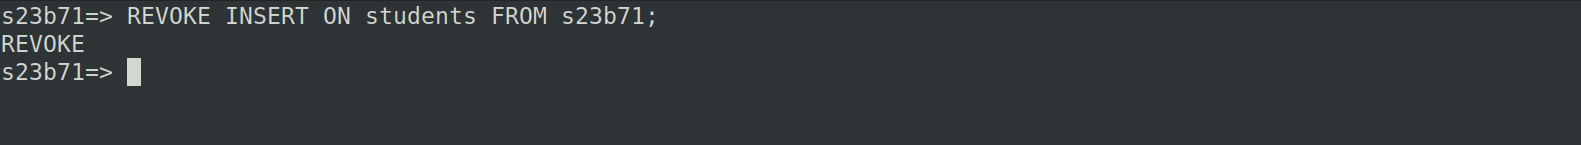
\includegraphics[width=\textwidth]{cycle4/4.1.1.png}
\end{figure}

\subsection*{1.b. Grant the permission to the user for inserting values in to students table and check whether insertion is possible or not}
Query:
\begin{Verbatim}[frame=single,framerule=1pt,fontfamily=courier,fontsize=\small]
GRANT INSERT ON students TO s23b71;
\end{Verbatim}
\begin{figure}[H]
    \centering
    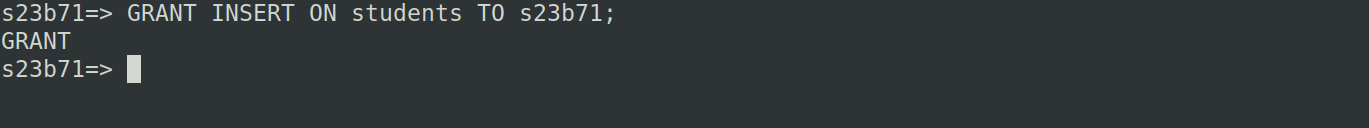
\includegraphics[width=\textwidth]{cycle4/4.1.2.png}
\end{figure}

\subsection*{2.a. Start a new transaction and insert a row into the Staff table. Commit the transaction and display the changes to the table}
Query:
\begin{Verbatim}[frame=single,framerule=1pt,fontfamily=courier,fontsize=\small]
BEGIN TRANSACTION;
INSERT INTO STAFF VALUES (6, 'Chris', 'White', '5 St', 'City5', 'ST', 
10005, 127, 1115555, '2022-05-01', 35000, 'Lecturer');
COMMIT;
SELECT * FROM STAFF;
\end{Verbatim}
\begin{figure}[H]
    \centering
    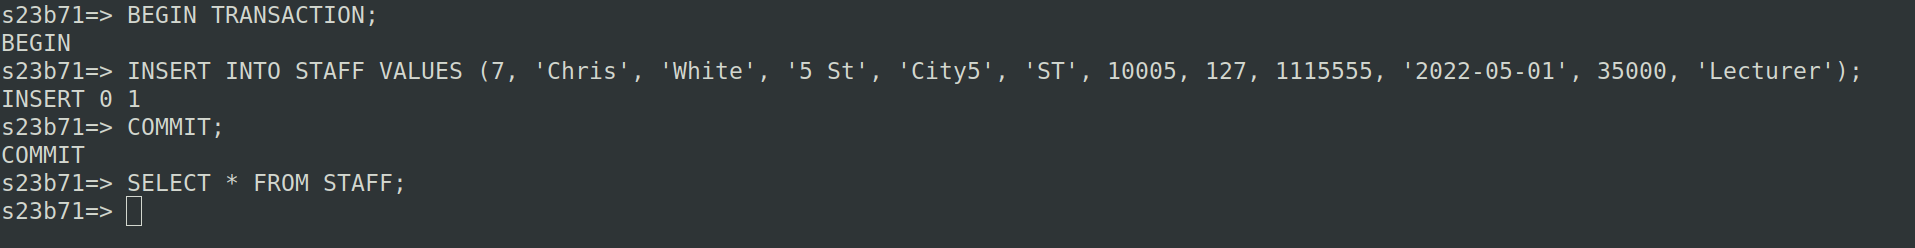
\includegraphics[width=\textwidth]{cycle4/4.2.1.png}
\end{figure}
\begin{figure}[H]
    \centering
    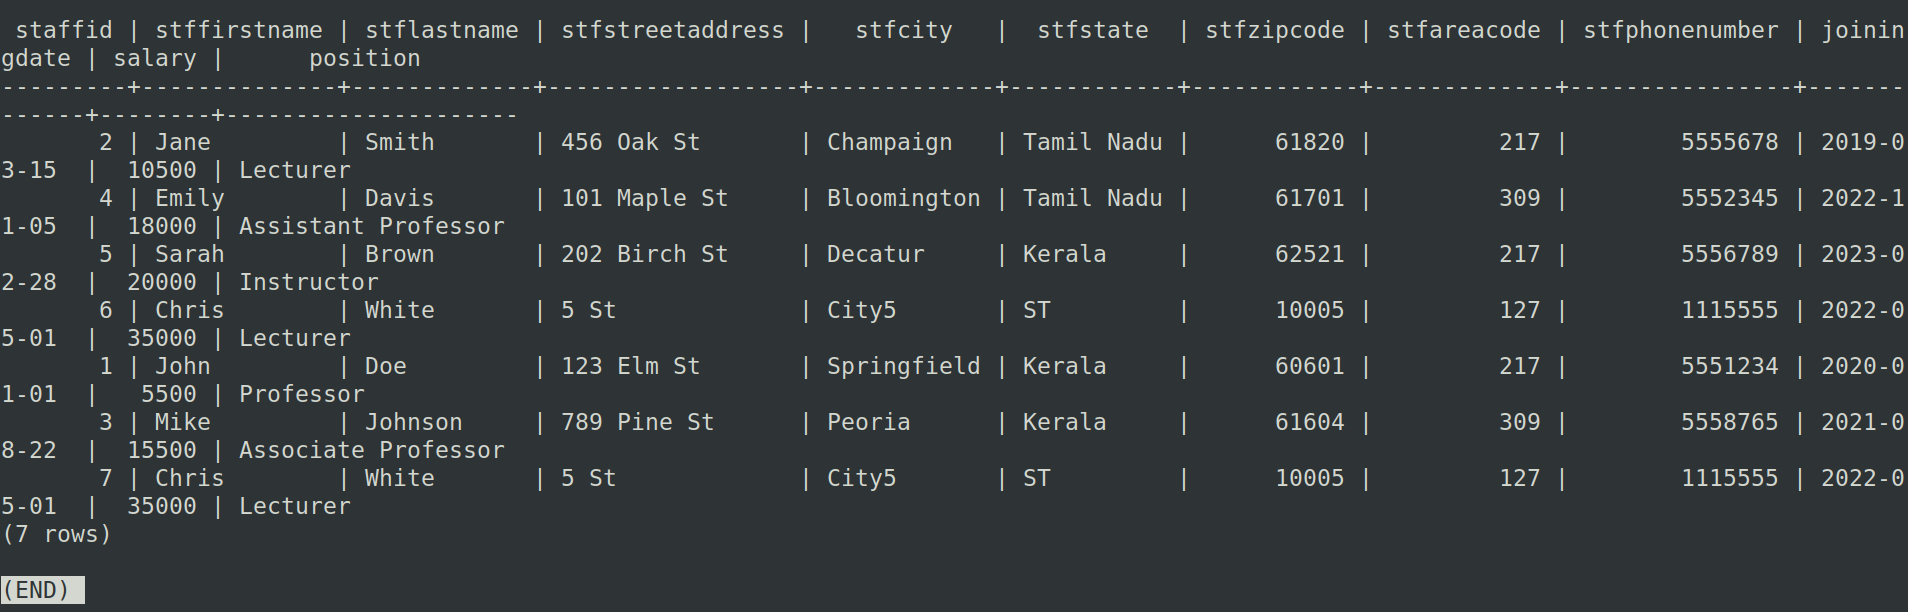
\includegraphics[width=\textwidth]{cycle4/4.2.2.png}
\end{figure}

\subsection*{2.b. Start a new transaction and insert a row into the Staff table.Undo the transaction and display the changes to the table}
Query:
\begin{Verbatim}[frame=single,framerule=1pt,fontfamily=courier,fontsize=\small]
BEGIN TRANSACTION;
INSERT INTO STAFF VALUES (7, 'Anna', 'White', '5 St', 'City5', 'ST', 
10005, 127, 1115555, '2022-05-01', 35000, 'Lecturer');
SELECT * FROM STAFF;
ROLLBACK;
SELECT * FROM STAFF;
\end{Verbatim}
\begin{figure}[H]
    \centering
    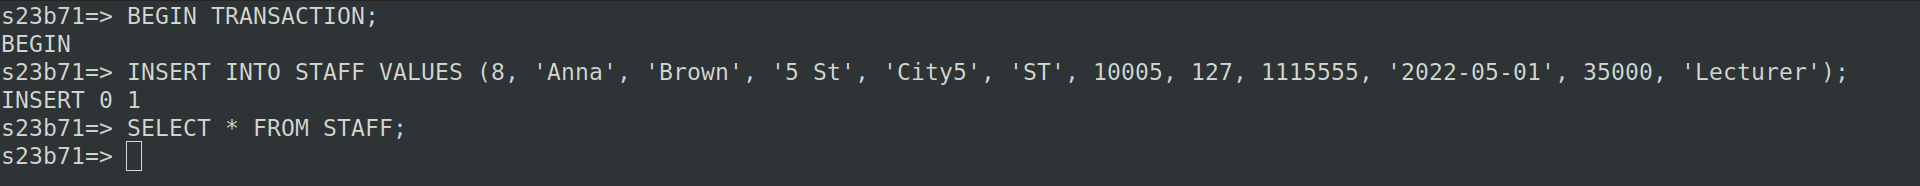
\includegraphics[width=\textwidth]{cycle4/4.2.3.png}
\end{figure}
\begin{figure}[H]
    \centering
    \includegraphics[width=\textwidth]{cycle4/4.2.4.png}
\end{figure}

\subsection*{3. Display the staffid and title for Faculty along with staffid and position for Staff in a single table. Indicate the source of the row in the result by adding an additional column EMPLOYEE with possible values as 'F' (Faculties) and 'S' (Staff). Display all rows (Using UNION ALL)}
Query:
\begin{Verbatim}[frame=single,framerule=1pt,fontfamily=courier,fontsize=\small]
SELECT staffid,title AS role, 'F' AS EMPLOYEE FROM faculty 
UNION ALL 
SELECT staffid,position AS role, 'S' AS EMPLOYEE FROM staff;
\end{Verbatim}
\begin{figure}[H]
    \centering
    \includegraphics[width=\textwidth]{cycle4/4.3.png}
\end{figure}

\subsection*{4. Find the pass percentage of a particular subject (using grade)}
Query:
\begin{Verbatim}[frame=single,framerule=1pt,fontfamily=courier,fontsize=\small]
SELECT classid,
100.0 * COUNT
(
    CASE WHEN grade NOT IN ('F') THEN -5 END
) 
/ COUNT(*)
AS PASSPERCENTAGE
FROM student_schedules
GROUP BY classid
ORDER BY classid;
\end{Verbatim}

\subsection*{5. Display the number of students in each classroom on a particular building using JOINS}
Query:
\begin{Verbatim}[frame=single,framerule=1pt,fontfamily=courier,fontsize=\small]
SELECT buildingcode,buildingname,classroomid,COUNT(studentid) 
FROM classes NATURAL JOIN classrooms NATURAL JOIN buildings 
NATURAL JOIN student_schedules 
GROUP BY buildingcode,buildingname,classroomid 
ORDER BY classroomid;
\end{Verbatim}
\begin{figure}[H]
    \centering
    \includegraphics[width=\textwidth]{cycle4/4.5.png}
\end{figure}

\subsection*{6. Display the list of students and staff who have the same zip code}
Query:
\begin{Verbatim}[frame=single,framerule=1pt,fontfamily=courier,fontsize=\small]
SELECT s1.studfirstname,s1.studlastname,s2.stffirstname,
s2.stflastname,s1.studzipcode 
FROM students s1 JOIN staff s2 ON s1.studzipcode = s2.stfzipcode;
\end{Verbatim}
\begin{figure}[H]
    \centering
    \includegraphics[width=\textwidth]{cycle4/4.6.png}
\end{figure}

\subsection*{7. Display the list of faculty who engage same subject (for any particular subject name)}
Query:
\begin{Verbatim}[frame=single,framerule=1pt,fontfamily=courier,fontsize=\small]
SELECT stffirstname,stflastname,staffid,subjectname,subjectcode 
FROM staff NATURAL JOIN faculty_subjects NATURAL JOIN subjects 
WHERE subjectcode=101;
\end{Verbatim}
\begin{figure}[H]
    \centering
    \includegraphics[width=\textwidth]{cycle4/4.8.png}
\end{figure}

\subsection*{Result}
Query executed and output obtained successfully.

\newpage
\section*{\centering{Cycle 5}}

\subsection*{1. Create a view from faculty, staff and student relation to display faculty name, classid, subject name based on schedule given.}
Query:
\begin{Verbatim}[frame=single,framerule=1pt,fontfamily=courier,fontsize=\small]
CREATE VIEW faculty_schedule AS
SELECT s.stffirstname, s.stflastname, fc.classid, 
       sub.subjectname
FROM staff s
JOIN faculty f ON s.staffid = f.staffid
JOIN faculty_classes fc ON f.staffid = fc.staffid
JOIN classes c ON fc.classid = c.classid
JOIN subjects sub ON c.subjectid = sub.subjectid;

SELECT * FROM faculty_schedule;
\end{Verbatim}
\begin{figure}[H]
    \centering
    \includegraphics[width=\textwidth]{cycle5/5_1_1.png}
\end{figure}
\begin{figure}[H]
    \centering
    \includegraphics[width=\textwidth]{cycle5/5_1_2.png}
\end{figure}

\subsection*{2. Use assert statement to check whether Classroom table has at least 1 data}
Query:
\begin{Verbatim}[frame=single,framerule=1pt,fontfamily=courier,fontsize=\small]
DO $$
DECLARE
    row_count INT;
BEGIN
    SELECT COUNT(*) INTO row_count FROM classrooms;
    
    ASSERT row_count >= 1, 'Classroom table must have at least 1 data';
    
    RAISE NOTICE 'Assertion passed: Classroom table has % row(s)', 
                  row_count;
END $$;
\end{Verbatim}
\begin{figure}[H]
    \centering
    \includegraphics[width=\textwidth]{cycle5/5_2_1.png}
\end{figure}


\subsection*{3. Write a PL/SQL block to do the following:}
\subsubsection*{a. Using control structures, display the list of faculties who have been hired between two dates}
Query:
\begin{Verbatim}[frame=single,framerule=1pt,fontfamily=courier,fontsize=\small]
DO $$
DECLARE
    staff_record RECORD;
    start_date DATE := '2020-01-01';
    end_date DATE := '2022-12-31';
BEGIN
    RAISE NOTICE 'Faculties hired between % and %:', 
                  start_date, end_date;
    RAISE NOTICE '--------------------------------------------';
    
    FOR staff_record IN 
        SELECT s.staffid, s.stffirstname, s.stflastname, 
               s.joiningdate, f.title
        FROM staff s
        JOIN faculty f ON s.staffid = f.staffid
        WHERE s.joiningdate BETWEEN start_date AND end_date
        ORDER BY s.joiningdate
    LOOP
        RAISE NOTICE 'ID: %, Name: % %, Title: %, Hired: %',
            staff_record.staffid,
            staff_record.stffirstname,
            staff_record.stflastname,
            staff_record.title,
            staff_record.joiningdate;
    END LOOP;
END $$;
\end{Verbatim}
\begin{figure}[H]
    \centering
    \includegraphics[width=\textwidth]{cycle5/5_3_a.png}
\end{figure}

\subsubsection*{b. Using CASE statement, satisfy the following conditions accepting Staff ID as input:}
\subsubsection*{i. Case 1: if salary < 5000, give 50\% increment}
\subsubsection*{ii. Case 2: if salary between 5000 and 10000, give 10\% increment}
\subsubsection*{iii. Case 3: if salary > 10000, display a message 'No Increment'}
Query:
\begin{Verbatim}[frame=single,framerule=1pt,fontfamily=courier,fontsize=\small]
DO $$
DECLARE
    input_staffid INT := 5;
    current_salary INT;
    new_salary INT;
    increment_msg TEXT;
BEGIN
    SELECT salary INTO current_salary 
    FROM staff 
    WHERE staffid = input_staffid;
    
    IF current_salary IS NULL THEN
        RAISE NOTICE 'Staff ID % not found', input_staffid;
        RETURN;
    END IF;
    
    CASE
        WHEN current_salary < 5000 THEN
            new_salary := current_salary * 1.5;
            increment_msg := '50% increment applied';
        WHEN current_salary BETWEEN 5000 AND 10000 THEN
            new_salary := current_salary * 1.1;
            increment_msg := '10% increment applied';
        WHEN current_salary > 10000 THEN
            new_salary := current_salary;
            increment_msg := 'No Increment';
    END CASE;
    
    RAISE NOTICE 'Staff ID: %', input_staffid;
    RAISE NOTICE 'Current Salary: %', current_salary;
    RAISE NOTICE 'New Salary: %', new_salary;
    RAISE NOTICE 'Status: %', increment_msg;
END $$;
\end{Verbatim}
\begin{figure}[H]
    \centering
    \includegraphics[width=\textwidth]{cycle5/5_3_b.png}
\end{figure}

\subsubsection*{c. Read the Faculty table row by row using WHILE loop and display the last name of the faculty (Example: 'Last Name: Antony')}
Query:
\begin{Verbatim}[frame=single,framerule=1pt,fontfamily=courier,fontsize=\small]
DO $$
DECLARE
    faculty_cursor CURSOR FOR 
        SELECT s.stflastname 
        FROM staff s 
        JOIN faculty f ON s.staffid = f.staffid;
    last_name VARCHAR(30);
    row_count INT := 0;
BEGIN
    RAISE NOTICE 'Faculty Last Names:';
    RAISE NOTICE '--------------------';
    
    OPEN faculty_cursor;
    
    LOOP
        FETCH faculty_cursor INTO last_name;
        EXIT WHEN NOT FOUND;
        
        row_count := row_count + 1;
        RAISE NOTICE 'Last Name: %', last_name;
    END LOOP;
    
    CLOSE faculty_cursor;
    
    RAISE NOTICE '--------------------';
    RAISE NOTICE 'Total Faculty: %', row_count;
END $$;
\end{Verbatim}
\begin{figure}[H]
    \centering
    \includegraphics[width=\textwidth]{cycle5/5_3_c.png}
\end{figure}

\subsection*{Result}
Query executed and output obtained successfully.

\newpage
\section*{\centering{Cycle 6}}
\subsection*{TRIGGERS \& CURSORS}

\subsection*{Triggers:}

\subsubsection*{1. Create a trigger such that before a row is deleted from Student\_Schedules table, it is inserted into another table}
Query:
\begin{Verbatim}[frame=single,framerule=1pt,fontfamily=courier,fontsize=\small]
-- Create backup table
CREATE TABLE student_schedules_backup (
    classid INT,
    studentid INT,
    classstatus INT,
    grade VARCHAR(30),
    deleted_at TIMESTAMP DEFAULT CURRENT_TIMESTAMP
);

-- Create trigger function
CREATE OR REPLACE FUNCTION backup_student_schedule()
RETURNS TRIGGER AS $$
BEGIN
    INSERT INTO student_schedules_backup 
        (classid, studentid, classstatus, grade)
    VALUES 
        (OLD.classid, OLD.studentid, OLD.classstatus, OLD.grade);
    RETURN OLD;
END;
$$ LANGUAGE plpgsql;

-- Create trigger
CREATE TRIGGER before_delete_student_schedule
BEFORE DELETE ON student_schedules
FOR EACH ROW
EXECUTE FUNCTION backup_student_schedule();

-- Test the trigger
DELETE FROM student_schedules WHERE classid = 1 AND studentid = 1;
SELECT * FROM student_schedules_backup;
\end{Verbatim}
\begin{figure}[H]
    \centering
    \includegraphics[width=\textwidth]{cycle6/6-1.png}
\end{figure}

\subsubsection*{2. Create a trigger on Students table in which it stops deletion and updation on Sundays and allows insertion only on Fridays}
Query:
\begin{Verbatim}[frame=single,framerule=1pt,fontfamily=courier,fontsize=\small]
-- Create trigger function
CREATE OR REPLACE FUNCTION restrict_student_operations()
RETURNS TRIGGER AS $$
BEGIN
    -- Check for DELETE or UPDATE on Sunday
    IF (TG_OP = 'DELETE' OR TG_OP = 'UPDATE') AND 
       EXTRACT(DOW FROM CURRENT_DATE) = 0 THEN
        RAISE EXCEPTION 'DELETE and UPDATE operations are not allowed 
                         on Sundays';
    END IF;
    
    -- Check for INSERT only on Friday
    IF TG_OP = 'INSERT' AND EXTRACT(DOW FROM CURRENT_DATE) != 5 THEN
        RAISE EXCEPTION 'INSERT operation is only allowed on Fridays';
    END IF;
    
    IF TG_OP = 'DELETE' THEN
        RETURN OLD;
    ELSE
        RETURN NEW;
    END IF;
END;
$$ LANGUAGE plpgsql;

-- Create trigger
CREATE TRIGGER student_day_restriction
BEFORE INSERT OR UPDATE OR DELETE ON students
FOR EACH ROW
EXECUTE FUNCTION restrict_student_operations();

-- Test the trigger (will succeed/fail based on current day)
-- INSERT INTO students VALUES (6, 'Test', 'User', '123 St', 
--     'City', 'ST', 12345, 123, '1234567890');
\end{Verbatim}
\begin{figure}[H]
    \centering
    \includegraphics[width=\textwidth]{cycle6/6-2.png}
\end{figure}

\newpage
\subsubsection*{3. Write a trigger on Staff table such that updation is not possible if new salary is greater than old salary}
Query:
\begin{Verbatim}[frame=single,framerule=1pt,fontfamily=courier,fontsize=\small]
-- Create trigger function
CREATE OR REPLACE FUNCTION prevent_salary_increase()
RETURNS TRIGGER AS $$
BEGIN
    IF NEW.salary > OLD.salary THEN
        RAISE EXCEPTION 'Salary cannot be increased. 
                         Old salary: %, New salary: %', 
                         OLD.salary, NEW.salary;
    END IF;
    RETURN NEW;
END;
$$ LANGUAGE plpgsql;

-- Create trigger
CREATE TRIGGER no_salary_increase
BEFORE UPDATE ON staff
FOR EACH ROW
EXECUTE FUNCTION prevent_salary_increase();

-- Test the trigger (should fail)
UPDATE staff SET salary = 60000 WHERE staffid = 1;

-- Test the trigger (should succeed - decreasing salary)
UPDATE staff SET salary = 45000 WHERE staffid = 5;
SELECT * FROM staff WHERE staffid = 5;
\end{Verbatim}
\begin{figure}[H]
    \centering
    \includegraphics[width=\textwidth]{cycle6/6-3.png}
\end{figure}

\subsection*{Cursors:}

\subsubsection*{1. Write a PL/SQL block to display the details of Staff living in a particular city}
Query:
\begin{Verbatim}[frame=single,framerule=1pt,fontfamily=courier,fontsize=\small]
DO $$
DECLARE
    staff_cursor CURSOR FOR 
        SELECT staffid, stffirstname, stflastname, 
               stfstreetaddress, stfcity, stfstate, 
               stfzipcode, stfphonenumber
        FROM staff
        WHERE stfcity = 'Springfield';
    staff_record RECORD;
    count_staff INT := 0;
BEGIN
    RAISE NOTICE 'Staff Members Living in Springfield:';
    RAISE NOTICE '=========================================';
    
    OPEN staff_cursor;
    
    LOOP
        FETCH staff_cursor INTO staff_record;
        EXIT WHEN NOT FOUND;
        
        count_staff := count_staff + 1;
        RAISE NOTICE 'Staff ID: %', staff_record.staffid;
        RAISE NOTICE 'Name: % %', staff_record.stffirstname, 
                     staff_record.stflastname;
        RAISE NOTICE 'Address: %, %, % - %', 
                     staff_record.stfstreetaddress,
                     staff_record.stfcity,
                     staff_record.stfstate,
                     staff_record.stfzipcode;
        RAISE NOTICE 'Phone: %', staff_record.stfphonenumber;
        RAISE NOTICE '-----------------------------------------';
    END LOOP;
    
    CLOSE staff_cursor;
    
    RAISE NOTICE 'Total Staff in Springfield: %', count_staff;
END $$;
\end{Verbatim}
\begin{figure}[H]
    \centering
    \includegraphics[width=\textwidth]{cycle6/6-4.png}
\end{figure}

\newpage
\subsubsection*{2. Using parameterized cursors list the name of staff who work in the same department in which 'xyz' works}
Query:
\begin{Verbatim}[frame=single,framerule=1pt,fontfamily=courier,fontsize=\small]
DO $$
DECLARE
    target_staff VARCHAR(30) := 'John';
    target_dept INT;
    staff_cursor CURSOR (dept_id INT) FOR
        SELECT DISTINCT s.staffid, s.stffirstname, s.stflastname, 
               c.departmentid, c.categorydescription
        FROM staff s
        JOIN faculty_subjects fs ON s.staffid = fs.staffid
        JOIN subjects sub ON fs.subjectid = sub.subjectid
        JOIN categories c ON sub.categoryid = c.categoryid
        WHERE c.departmentid = dept_id
        ORDER BY s.staffid;
    staff_record RECORD;
BEGIN
    -- Find department of target staff
    SELECT DISTINCT c.departmentid INTO target_dept
    FROM staff s
    JOIN faculty_subjects fs ON s.staffid = fs.staffid
    JOIN subjects sub ON fs.subjectid = sub.subjectid
    JOIN categories c ON sub.categoryid = c.categoryid
    WHERE s.stffirstname = target_staff
    LIMIT 1;
    
    IF target_dept IS NULL THEN
        RAISE NOTICE 'Staff member % not found or not assigned 
                      to any department', target_staff;
        RETURN;
    END IF;
    
    RAISE NOTICE 'Staff in Department % (same as %):',
                 target_dept, target_staff;
    RAISE NOTICE '==========================================';
    
    FOR staff_record IN staff_cursor(target_dept) LOOP
        RAISE NOTICE 'ID: %, Name: % %, Department: %, 
                      Category: %',
            staff_record.staffid,
            staff_record.stffirstname,
            staff_record.stflastname,
            staff_record.departmentid,
            staff_record.categorydescription;
    END LOOP;
END $$;
\end{Verbatim}
\begin{figure}[H]
    \centering
    \includegraphics[width=\textwidth]{cycle6/6-5.png}
\end{figure}

\subsubsection*{3. Write a PL/SQL block to display Staff\_ID and salary of two highest paid staffs using cursors}
Query:
\begin{Verbatim}[frame=single,framerule=1pt,fontfamily=courier,fontsize=\small]
DO $$
DECLARE
    staff_cursor CURSOR FOR
        SELECT staffid, stffirstname, stflastname, salary
        FROM staff
        ORDER BY salary DESC
        LIMIT 2;
    staff_record RECORD;
    rank_num INT := 0;
BEGIN
    RAISE NOTICE 'Top 2 Highest Paid Staff Members:';
    RAISE NOTICE '==================================';
    
    FOR staff_record IN staff_cursor LOOP
        rank_num := rank_num + 1;
        RAISE NOTICE 'Rank #%', rank_num;
        RAISE NOTICE 'Staff ID: %', staff_record.staffid;
        RAISE NOTICE 'Name: % %', staff_record.stffirstname,
                     staff_record.stflastname;
        RAISE NOTICE 'Salary: %', staff_record.salary;
        RAISE NOTICE '----------------------------------';
    END LOOP;
END $$;
\end{Verbatim}
\begin{figure}[H]
    \centering
    \includegraphics[width=\textwidth]{cycle6/6-6.png}
\end{figure}

\subsection*{Result}
Query executed and output obtained successfully.

\newpage
\section*{\centering{Cycle 7}}
\subsection*{MongoDB Queries}

\subsubsection*{1. Create a database named College and a collection named Students. Insert at least 5 student documents.}
Query:
\begin{Verbatim}[frame=single,framerule=1pt,fontfamily=courier,fontsize=\small]
use College

db.students.insertMany([
  {RollNo: 101, Name: 'John Doe', Age: 22, Mark: 90, 
   Department: 'ECE'},
  {RollNo: 102, Name: 'Emily White', Age: 25, Mark: 60, 
   Department: 'CSE'},
  {RollNo: 70, Name: 'Jack Brown', Age: 20, Mark: 90, 
   Department: 'ECE'},
  {RollNo: 103, Name: 'Shravan Nander Pandala', Age: 20, Mark: 90, 
   Department: 'CSE'},
  {RollNo: 105, Name: 'Alice Green', Age: 19, Mark: 75, 
   Department: 'ECE'}
])
\end{Verbatim}
\begin{figure}[H]
    \centering
    \includegraphics[width=\textwidth]{cycle7/7.1.png}
\end{figure}

\subsubsection*{2. Retrieve all students.}
Query:
\begin{Verbatim}[frame=single,framerule=1pt,fontfamily=courier,fontsize=\small]
db.students.find()
\end{Verbatim}
\begin{figure}[H]
    \centering
    \includegraphics[width=\textwidth]{cycle7/7.2.png}
\end{figure}

\subsubsection*{3. Retrieve only name and department.}
Query:
\begin{Verbatim}[frame=single,framerule=1pt,fontfamily=courier,fontsize=\small]
db.students.find({RollNo:101},{_id:false,Name:true,Department:true})
\end{Verbatim}
\begin{figure}[H]
    \centering
    \includegraphics[width=\textwidth]{cycle7/7.3.png}
\end{figure}

\subsubsection*{4. Find student with roll\_no = 103.}
Query:
\begin{Verbatim}[frame=single,framerule=1pt,fontfamily=courier,fontsize=\small]
db.students.find({RollNo:103})
\end{Verbatim}
\begin{figure}[H]
    \centering
    \includegraphics[width=\textwidth]{cycle7/7.4.png}
\end{figure}

\subsubsection*{5. Update marks of roll\_no = 101.}
Query:
\begin{Verbatim}[frame=single,framerule=1pt,fontfamily=courier,fontsize=\small]
db.students.updateOne({RollNo:101},{$set:{Mark:80}})
\end{Verbatim}
\begin{figure}[H]
    \centering
    \includegraphics[width=\textwidth]{cycle7/7.5.png}
\end{figure}

\subsubsection*{6. Delete student with roll\_no = 105.}
Query:
\begin{Verbatim}[frame=single,framerule=1pt,fontfamily=courier,fontsize=\small]
db.students.findOneAndDelete({RollNo:105})
\end{Verbatim}
\begin{figure}[H]
    \centering
    \includegraphics[width=\textwidth]{cycle7/7.6.png}
\end{figure}

\subsubsection*{7. Students with marks > 70.}
Query:
\begin{Verbatim}[frame=single,framerule=1pt,fontfamily=courier,fontsize=\small]
db.students.find({Mark:{$gt:70}})
\end{Verbatim}
\begin{figure}[H]
    \centering
    \includegraphics[width=\textwidth]{cycle7/7.7.png}
\end{figure}

\subsubsection*{8. Students aged between 18 and 22.}
Query:
\begin{Verbatim}[frame=single,framerule=1pt,fontfamily=courier,fontsize=\small]
db.students.find({Age:{$gt:18,$lt:22}})
\end{Verbatim}
\begin{figure}[H]
    \centering
    \includegraphics[width=\textwidth]{cycle7/7.8.png}
\end{figure}

\subsubsection*{9. Students sorted by marks (descending).}
Query:
\begin{Verbatim}[frame=single,framerule=1pt,fontfamily=courier,fontsize=\small]
db.students.find().sort({Mark:-1})
\end{Verbatim}
\begin{figure}[H]
    \centering
    \includegraphics[width=\textwidth]{cycle7/7.9.png}
\end{figure}

\subsubsection*{10. Count students in ECE.}
Query:
\begin{Verbatim}[frame=single,framerule=1pt,fontfamily=courier,fontsize=\small]
db.students.countDocuments({Department:'ECE'})
\end{Verbatim}
\begin{figure}[H]
    \centering
    \includegraphics[width=\textwidth]{cycle7/7.10.png}
\end{figure}

\subsection*{Result}
Query executed and output obtained successfully.

\end{document}
